\chapter{Pattern Matching su Stringhe}
\section{Introduzione}
Il problema del pattern matching consiste cercare un motivo all'interno di un
oggetto più o meno complesso. In questo corso ci si concentrerà sul pattern matching
su stringhe, ovvero cercare all'interno di un testo $T$ le occorrenze di un
pattern $P$.
\begin{definizione}[\textbf{Stringa}]
    Definiamo una \textbf{stringa} $X$ come una giustapposizione di simboli
    appartenenti a un alfabeto $\Sigma$.
    \begin{equation}
        X=x_1x_2\dots x_n \ \ x_i \in \Sigma \ \forall i = 1, \dots, n
    \end{equation}
    In aggiunta, definiremo:
    \begin{itemize}
        \item \textbf{Stringa nulla} $\varepsilon$ è una stringa composta da
              zero simboli.
        \item Simbolo in posizione $i$ si riferisce al simbolo in posizione
              $i$-esima $x_i = X[i]$
        \item \textbf{Sottostringa} da $i$ a $j$ è una porzione di stringa
              compresa tra gli indici $i$ e $j$.
              \begin{equation}
                  X[i, j] = X[i:j] = X[i]X[i+1]\dots X[j - 1]X[j]
              \end{equation}
              Posso esprimerlo attraverso la seguente notazione: $X[i, j] \lor X[i:j]$.
              Possiamo dire che una sottostringa $X[i, j]$ si definisce:
              \begin{itemize}
                  \item \textbf{Propria} se $i \neq 1 \land j \neq |X|$.
                  \item \textbf{Impropria} altrimenti.
              \end{itemize}
        \item \textbf{Prefisso} di lunghezza $j$ è una sottostringa $X[1, j]$.
              Anche in questo caso possiamo distinguere:
              \begin{itemize}
                  \item \textbf{Proprio} se $j \neq |X|$
                  \item \textbf{Improprio} altrimenti.
              \end{itemize}
              Per il prefisso è possibile definire anche il prefisso nullo, ovvero il
              prefisso composto da zero caratteri ($X[1, j]=\varepsilon \ \to \ j = 0$).
        \item \textbf{Suffisso} che inizia in $i$ è la sottostringa $X[i,|X|]$.
              Di questa sottostringa posso calcolare la lunghezza del prefisso come:
              \begin{equation}
                  |X[i,|X|]| = |X| - i + 1
              \end{equation}
              Anche in questo caso possiamo distinguere:
              \begin{itemize}
                  \item \textbf{Proprio} se $i \neq 1$
                  \item \textbf{Improprio} altrimenti.
              \end{itemize}
              È possibile definire il suffisso nullo ovvero quello composto da zero
              caratteri ($X[i,|X|]=\varepsilon \ \to \ i = |X| + 1$).
    \end{itemize}
\end{definizione}
\begin{nota}
    Una \textbf{stringa} di caratteri si differenzia da un \textbf{sequenza}
    degli stessi caratteri dal momento che:
    \begin{itemize}
        \item \textbf{stringa}: è una giustapposizione di caratteri, quindi sono
              tutti concatenati
              \begin{equation}
                  X = \sigma_1\sigma_2\dots\sigma_n
              \end{equation}
        \item \textbf{sequenza}: è un elenco di caratteri separati da un separatore
              \begin{equation}
                  X= \langle\sigma_1,\sigma_2,\dots,\sigma_n\rangle
              \end{equation}
    \end{itemize}
\end{nota}
Quando si parla di string matching possiamo definire due tipi. Dati un pattern
$P$ e un testo $T$ possiamo definire lo string matching:
\begin{enumerate}
    \item \textbf{Esatto}: consiste nel cercare le occorrenze esatte di $P$ in $T$.
    \item \textbf{Approssimato}: consiste nel cercare le occorrenze approssimate
          di $P$ in $T$.
\end{enumerate}
\subsection{String Matching Esatto}
Possiamo definire il problema di \textbf{string matching esatto} formalmente nel
seguente modo:
\begin{itemize}
    \item \textbf{input}: un testo $T$ e un pattern $P$, rispettivamente
          $|T|=n$ e $|P|=m$, definiti su un alfabeto $\Sigma$.
    \item \textbf{output}: tutte le occorrenze esatte $i$ di $T$ ($T[i,i+m-1]=P$).
\end{itemize}
\begin{definizione}[\textbf{Occorrenza esatta}]
    Una posizione $i$ del testo $T$ tale che $T[i, i + m - 1] = P$ è
    un'\textbf{occorrenza esatta} di $P$ in $T$.
\end{definizione}
\begin{definizione}[\textbf{Match}]
    Dati due simboli $s_1, s_2 \in \Sigma$ si ha un \textbf{match} se $s_1 = s_2$.
\end{definizione}
\begin{definizione}[\textbf{Mismatch}]
    Dati due simboli $s_1, s_2 \in \Sigma$ si ha un \textbf{mismatch} se $s_1
        \neq s_2$.
\end{definizione}
Avendo definito il problema in questo modo è possibile definire un semplice
algoritmo che mi permette di calcolare l'output del problema. Questo algoritmo
utilizza una finestra $W$, delle stesse dimensioni del pattern, che scorre sul
testo. L'algoritmo semplice che permette di calcolare le occorrenze esatte è:
\begin{enumerate}
    \item Uso una finestra $W$ lunga $m$ che scorre lungo $T$ da sinistra a
          destra. La posizione iniziale di $W$ è $i = 1$.
    \item Si confronta ogni simbolo di $P$ con il corrispondente simbolo di $T$
          all'interno di $W$ da sinistra verso destra.
          \begin{equation}
              P[j] = T[i + j - 1] \ \forall \ j \ \text{tale che} \ 1 \leq j
              \leq m \ \Rightarrow T[i, i + m - 1] = P
          \end{equation}
    \item $W$ viene spostata di una posizione verso destra e il confronto viene
          ripetuto.
    \item Ultima posizione di $W$ è $i = |T| - |P| + 1 = n - m + 1$
\end{enumerate}
\begin{algorithm}
    \begin{algorithmic}
        \Function{trivial\_exact\_occurrences}{$T, P$}
        \State $n\gets |T|$
        \State $m \gets |P|$
        \State $i\gets 1$
        \While {$i \leq n - m + 1$}
        \State $j \gets 1$
        \While {$P[j] = T[i + j - 1] \ \land \ j \leq m$}
        \State $j \leq j + 1$
        \EndWhile
        \If {$j = m + 1$}
        \State $\text{output } i$
        \EndIf
        \State $i \gets i + 1$
        \EndWhile
        \EndFunction
    \end{algorithmic}
    \caption{Algoritmo banale per String Matching Esatto}
\end{algorithm}
Questo algoritmo richiede un tempo pari a $\mathcal{O}(m \cdot n)$.
\begin{nota}
    Questo algoritmo può essere migliorato spostando la finestra alla posizione
    successiva al primo mismatch oppure si può effettuare un preprocessing del
    pattern e del testo, permettendo di passare da una complessità quadratica ad
    una logaritmica o lineare.
\end{nota}
\subsection{String Matching Approssimato}
Definiremo il problema di \textbf{string matching approssimato} formalmente nel
seguente modo:
\begin{itemize}
    \item \textbf{input}: testo $T$ e un pattern $P$, rispettivamente $|T| = n$ e
          $|P| = m$, definiti entrambi su un alfabeto $\Sigma$, infine, una
          soglia $k$ di errore.
    \item \textbf{output}: tutte le occorrenze approssimate di $P$ in $T$ che
          rispettano la soglia di errore $k$.
\end{itemize}
Introducendo una soglia di errore abbiamo bisogno di definire una metrica per
calcolare l'errore. Per fare ciò si utilizza la \textit{distanza di edit} (ED)
tra due stringhe. Tale distanza è definita come il minimo numero di operazioni di
sostituzione, cancellazione, inserimento di un simbolo che trasformano una
stringa nell'altra.
\begin{nota}
    \begin{equation}
        ED(X_1, X_2) \geq abs(|X_1| - |X_2|)
    \end{equation}
\end{nota}
\begin{definizione}[\textbf{Occorrenza approssimata}]
    Una posizione $i$ del testo $T$, tale che esista almeno una sottostringa
    $S = T[i - L + 1,i]$, con $ED(P, S) \leq k$, che è un'occorrenza approssimata
    di $P$ in $T$.
\end{definizione}
\begin{nota}
    Si può aggiungere:
    \begin{enumerate}
        \item Se $ED(P, S) \leq k$, allora $i$ è occorrenza approssimata.
        \item $ED(P, S) \geq abs(m - L) \ \Rightarrow \ $se $abs(m - L) > k$
              allora $i$ non può essere occorrenza approssimata.
    \end{enumerate}
\end{nota}
Quindi il problema formale dello \textbf{string matching approssimato} verrà
definito come:
\begin{itemize}
    \item \textbf{input}: un testo $T$ e un pattern $P$, rispettivamente $|T| = n$
          e $|P| = m$, definiti entrambi su un alfabeto $\Sigma$, infine, una
          soglia $k$ di errore.
    \item \textbf{output}: tutte le occorrenze approssimate di $P$ in $T$ tale
          che  $ED(P,S)\le k$.
\end{itemize}
Avendo definito il problema in questo modo è possibile definire un semplice
algoritmo che mi permette di calcolare l'output del problema. Questo algoritmo
utilizza una finestra $W$, di dimensione variabile, che scorre sul testo.
\begin{enumerate}
    \item Uso una finestra $W$ di lunghezza variabile $\in [m - k, m + k]$, per
          un totale di $2k+1$ ampiezze da testare, che scorre lungo il testo $T$ da
          sinistra a destra. La posizione iniziale di tale finestra è $i = m - k$ e
          la sua lunghezza iniziale è $m - k$.
    \item Se la distanza di edit tra $P$ e la sottostringa di $T$ compresa in $W$
          è $\leq \ k$, allora $i$ è occorrenza approssimata di $P$ in $T$.
    \item $W$ viene spostata a destra di una posizione.
\end{enumerate}
\begin{algorithm}
    \begin{algorithmic}
        \Function{trivial\_approx\_occurrences}{$T, P, k$}
        \State $n\gets |T|$
        \State $m \gets |P|$
        \State $i\gets m - k$
        \While {$i \leq n$}
        \State $L \gets  m - k$
        \While {$L \leq m + k \ \land \ i - L + 1 \geq 1$}
        \If {$ED(P, T[i - L + 1, i]) \leq k$}
        \State $\text{output } i$
        \EndIf
        \State $L \gets L + 1$
        \EndWhile
        \State $i \gets i + 1$
        \EndWhile
        \EndFunction
    \end{algorithmic}
    \caption{Algoritmo banale per String Matching Approssimato}
\end{algorithm}
Questo algoritmo mi permette di calcolare il matching approssimato in tempo
$\mathcal{O}(n \cdot k \cdot m^2)$, dove $m^2$ è dovuto al calcolo della distanza
di edit tra le due sottostringhe.
\section{Ricerca esatta con Automa a Stati Finiti}
Un automa è un modello di calcolo che riconosce un linguaggio, ovvero un insieme
di stringhe che godono di una proprietà. Gli automi a stati finiti riconoscono
un linguaggio regolare.
\begin{definizione} [\textbf{Automa a stati finiti}]
    Un \textbf{Automa a Stati Finiti} è formalmente una quintupla:
    \begin{equation}
        A = (Q, \ \Sigma, \ \delta, \ q_0, \ F)
    \end{equation}
    dove:
    \begin{itemize}
        \item $Q$, insieme \textit{finito} di stati.
        \item $\Sigma$, alfabeto in input.
        \item $\delta: Q \times \Sigma \to Q$, funzione di transizione, dove
              $\delta(q,\sigma)$ rappresenta lo stato di arrivo a partire da $q$
              dopo la lettura di $\sigma$.
        \item $q_0$, stato iniziale.
        \item $F$ (sottoinsieme di $Q$), insieme degli stati accettanti.
    \end{itemize}
\end{definizione}
Gli automi a stati finiti possono essere rappresentati attraverso un diagramma di
stato, ovvero attraverso una struttura a grafo dove i vertici sono gli stati.
Esiste l'arco $(q_1, q_2)$ se almeno un simbolo $\sigma$ è tale per cui $\delta
    (q_1,\sigma) = q_2$. L'arco $(q_1, q_2)$ viene etichettato dalla lista di
simboli che permettono la transizione da $q_1$ a $q_2$. Lo stato iniziale $q_0$
è indicato tramite un arco entrante che non esce da uno stato, mentre gli stati
accettanti sono indicati da un doppio bordo.

È possibile rappresentare la funzione di transizione $\delta$ degli automi
attraverso una matrice $T$ con $|Q|$ righe e $|\Sigma|$ colonne. Nella generica
cella $(q, \sigma)$ sarà contenuto il valore di $\delta(q, \sigma)$, ovvero lo
stato che raggiungo partendo dallo stato $q$ leggendo il simbolo $\sigma$.
\begin{equation}
    T[q,\sigma] = q' \iff \delta(q,\sigma) = q'
\end{equation}
\begin{definizione}[\textbf{Bordo}]
    Il \textbf{bordo} di una stringa $X$ è il più lungo prefisso \textbf{proprio}
    di $X$ che occorre come suffisso di $X$.
\end{definizione}
\begin{esempio}
    Esempi di bordo:
    \begin{itemize}
        \item $X = baaccbbaac$ il suo bordo sarà $B(X) = baac$
        \item $X = aaaccbbaac$ il suo bordo sarà $B(X) = \varepsilon$
        \item $X = abababa$ il suo bordo sarà $B(X) = ababa$
        \item $X = aaaaaaaa$ il suo bordo sarà $B(X) = aaaaaaa$
        \item $X = a$ il suo bordo sarà $B(X) = \varepsilon$
    \end{itemize}
\end{esempio}
\begin{nota}
    Il bordo di una stringa composta da un solo simbolo è sempre vuoto.
\end{nota}
\begin{definizione}[\textbf{Concatenazione}]
    La \textbf{concatenazione} di un simbolo $\sigma$ con la stringa $X$ è la
    stringa $X\sigma$.
\end{definizione}
Possiamo definire ora l'automa a stati finiti per la ricerca esatta di un pattern
$P$ di lunghezza $m$ definito su alfabeto $\Sigma$ come la quintupla $(Q, \Sigma,
    \delta, q_0, F)$ con:
\begin{itemize}
    \item $Q = \{0, 1, \dots, m\}$
    \item $\Sigma$ è l'alfabeto di definizione di $P$.
    \item $\delta: Q \times \Sigma \to Q$ è la funzione di transizione.
    \item $q_0 = 0$ è lo stato iniziale.
    \item $F = \{m\}$ è lo stato accettante.
\end{itemize}
A questo punto, il processo di ricerca esatta attraverso un automa a stati finiti
è composto da:
\begin{enumerate}
    \item \textbf{Preprocessing del pattern}: costruisco l'automa per il pattern
          $P$. Questo punto consiste nel calcolo della funzione di transizione
          $\delta$ in tempo $\theta(m \cdot |\Sigma|)$.
    \item \textbf{Ricerca nel testo}: uso dell'automa per riconoscere, in un testo
          $T$ definito su alfabeto $\Sigma$, tutte le occorrenze esatte di $P$.
          La scansione del testo $T$ avviene in tempo $\theta(n)$
\end{enumerate}
\subsection{Funzione di transizione}
La funzione di transizione $\delta$ per un pattern $P$ di lunghezza $m$ definito
su un alfabeto $\Sigma$ è definita per ogni $(j, \sigma) \in Q \times \Sigma$ tale
che $\delta(j, \sigma)$ è lo stato in cui si arriva da $j$ attraverso $\sigma$:
\begin{equation}
    \delta(j, \sigma) = \begin{cases}
        j + 1 & \text{se} \ j < m \ \land \ P[j + 1] = \sigma   \\
        k     & \text{se} \ j = m \ \lor \ P[j + 1] \neq \sigma
    \end{cases}
\end{equation}
dove $k$ è la lunghezza del bordo del prefisso di $P$ di lunghezza $1, j$ a cui
è concatenato $\sigma$, ovvero:
\begin{equation}
    k = |B(P[1, j]\sigma)|, \ \text{con} \ k \leq j
\end{equation}
\begin{itemize}
    \item Dallo stato $0$ si arriva allo stato $0$ per qualsiasi simbolo diverso
          da $P[1]$.
    \item Dallo stato $0$ si arriva allo stato $1$ attraverso il simbolo $P[1]$.
    \item  Dallo stato $j = m$ si arriva sempre a uno stato $k \leq m$, dallo
          stato $m$ si può giungere quindi di nuovo allo stato $m$.
\end{itemize}
\subsubsection{Calcolo della funzione di transizione $\delta$}
L'algoritmo più semplice che permette di calcolare i valori della funzione di
transizione $\delta$ consiste nell'applicare la funzione di transizione $\delta$
per come è definita senza sfruttare i valori che sono già stati computati.
\begin{algorithm}
    \begin{algorithmic}
        \Function{Trivial-build-transition-function}{$P$}
        \State $m \gets |P|$
        \State $\delta \gets empty\_table (m + 1) \times | \Sigma|$
        \For{$j \gets 0 \ \text{to} \ m - 1$}
        \State $\delta(j, P[j + 1]) \gets j + 1$
        \EndFor
        \For{$j \gets 0 \ \text{to} \ m$}
        \For{$\sigma \in \Sigma$}
        \State $\delta(j, \sigma) \gets |B(P[1, j]\sigma)|$
        \EndFor
        \EndFor
        \State \Return $\delta$
        \EndFunction
    \end{algorithmic}
    \caption{Algoritmo banale per il calcolo della funzione di transizione $\delta$}
\end{algorithm}
Questo algoritmo richiede un tempo nel caso peggiore pari a $\mathcal{O}(m^3
    |\Sigma|)$, questo è dovuto al fatto che per calcolare il bordo è necessario
un tempo, nel caso peggiore pari a $\mathcal{O}(m^2)$.

Per migliorare i tempi cambieremo approccio, definiamo $\delta_j$ come la funzione
di transizione di $P[1, j]$, ovvero come una funzione:
\begin{equation}
    \delta_j: \{0, 1, \dots, j\} \times \Sigma \to \{0, 1, \dots, j\}
\end{equation}
per questa funzione possiamo definire due casi particolari:
\begin{itemize}
    \item $\delta_0$ ovvero la funzione di transizione di $P[1, 0]$ che per
          definizione è $\varepsilon$, quindi il valore di tale funzione è sempre
          $0$.
    \item $\delta_m$ ovvero la funzione di transizione di $P[1, m]$ la quale
          corrisponde precisamente alla funzione di transizione del pattern $P$.
\end{itemize}
Possiamo definire il calcolo della funzione di transizione $\delta$ per un pattern
$P$ di lunghezza $m$ utilizzando l'induzione nel seguente modo:
\begin{itemize}
    \item \textbf{Caso base}: calcolo $\delta_0$. Questo risulta banale in quanto
          il valore di $\delta_0$ è sempre $0$.
    \item \textbf{Passo induttivo}: calcolo $\delta_j$ da $\delta_{j - 1}$ in
          questo caso dobbiamo distinguere il caso in cui $j = 1$ e i restanti.
          \begin{itemize}
              \item Nel caso in cui $j = 1$, possiamo definire la funzione di
                    transizione come:
                    \begin{enumerate}
                        \item Prendo il valore $0$ contenuto nella cella della
                              riga $0$ di $\delta_0$ in corrispondenza del
                              simbolo $P[1]$.
                        \item Sostituisco il valore $0$ con il valore $1$ (stato
                              successivo a $0$).
                        \item Aggiungo una nuova riga (corrispondente allo stato
                              $1$)
                        \item Copio la riga che corrisponde allo stato $0$ nella
                              riga che corrisponde allo stato $1$.
                        \item Rinomino $\delta_0$ in $\delta_1$.
                    \end{enumerate}
              \item Mentre nel caso in cui $j \neq 1$ possiamo definire la
                    funzione di transizione come:
                    \begin{enumerate}
                        \item Prendo il valore $k$ contenuto nella cella della
                              riga $j - 1$ di $\delta_{j - 1}$ in corrispondenza
                              del simbolo $P[j]$
                        \item Sostituisco il valore $k$ con il valore $j$ (stato
                              successivo a $j - 1$)
                        \item Aggiungo una nuova riga (corrispondente allo stato
                              $j$)
                        \item Copio la riga che corrisponde allo stato $k$ nella
                              riga che corrisponde allo stato $j$
                        \item Rinomino $\delta_{j - 1}$ in $\delta_j$
                    \end{enumerate}
          \end{itemize}
\end{itemize}
\begin{nota}
    Dimostrazione tramite esempi su slide.
\end{nota}
Con queste informazioni possiamo definire un algoritmo che mi permette di calcolare
la funzione di transizione $\delta$ in tempo $\theta(m \cdot |\Sigma|)$. Tale
algoritmo sfrutta le informazioni precedentemente calcolate.
\begin{algorithm}[!ht]
    \begin{algorithmic}
        \Function{Build-transition-function}{$P$}
        \State $m \gets |P|$
        \State $\delta \gets empty\_table (m + 1) \times | \Sigma|$
        \For{$\sigma \in \Sigma$}
        \State $\delta(0, \sigma) \gets 0$
        \EndFor
        \For{$j \gets 1 \ \text{to} \ m$}
        \State $k \gets \delta(j - 1, P[j])$
        \State $\delta(j - 1, P[j]) \gets j$
        \For{$\sigma \in \Sigma$}
        \State $\delta(j, \sigma) \gets \delta(k, \sigma)$
        \EndFor
        \EndFor
        \State \Return $\delta$
        \EndFunction
    \end{algorithmic}
    \caption{Algoritmo per il calcolo della funzione di transizione $\delta$}
\end{algorithm}
\subsection{Scansione del testo}
La scansione del testo inizia da uno stato iniziale $j_0 = 0$. Partendo da questo
stato, leggo il simbolo in posizione $i$ del testo ($T[i]$) e mi sposto nello stato
$j_i$ attraverso la funzione di transizione $\delta(j_{i - 1}, T[i])$.
\begin{esempio}
    Consideriamo il testo $T$:
    \begin{table}[!ht]
        \centering
        \begin{tabular}{ccccccc}
            1                       & 2                      & 3
                                    & 4                      & 5
                                    & 6                      & 7 \\ \hline
            \multicolumn{1}{|c|}{c} & \multicolumn{1}{c|}{a} &
            \multicolumn{1}{c|}{b}  & \multicolumn{1}{c|}{a} &
            \multicolumn{1}{c|}{c}  & \multicolumn{1}{c|}{a} &
            \multicolumn{1}{c|}{b}                               \\ \hline
        \end{tabular}
    \end{table}

    e il pattern $P$:
    \begin{table}[!ht]
        \centering
        \begin{tabular}{ccccccc}
            1                       & 2                      & 3
                                    & 4                          \\ \hline
            \multicolumn{1}{|c|}{a} & \multicolumn{1}{c|}{c} &
            \multicolumn{1}{c|}{a}  & \multicolumn{1}{c|}{c}     \\ \hline
        \end{tabular}
    \end{table}

    Su cui è stata definita la seguente funzione di transizione $\delta$:
    \begin{table}[!ht]
        \centering
        \begin{tabular}{|>{\columncolor[HTML]{EFEFEF}}c |c|c|c|} \hline
            $\delta$                           &
            \cellcolor[HTML]{EFEFEF}\textbf{a} &
            \cellcolor[HTML]{EFEFEF}\textbf{b} &
            \cellcolor[HTML]{EFEFEF}\textbf{c}             \\ \hline
            \textbf{0}                         & 1 & 0 & 0 \\ \hline
            \textbf{1}                         & 1 & 0 & 2 \\ \hline
            \textbf{2}                         & 3 & 0 & 0 \\ \hline
            \textbf{3}                         & 1 & 0 & 4 \\ \hline
            \textbf{4}                         & 3 & 0 & 0 \\ \hline
        \end{tabular}
    \end{table}

    La scansione del testo $T$ cercando le occorrenze esatte del pattern $P$ mi
    permette di ottenere il risultato riportato in figura \ref{fig:scansione}
    \begin{figure}[!ht]
        \centering
        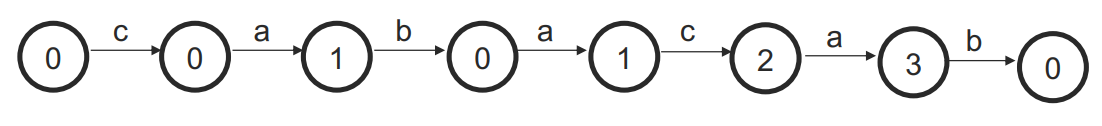
\includegraphics[width=0.5\textwidth]{img/pattern/ScansioneTesto.png}
        \caption{Risultato della scansione del testo}
        \label{fig:scansione}
    \end{figure}
\end{esempio}
A questo punto è necessario identificare un'occorrenza esatta del pattern $P$
nel testo $T$. Per risolvere questo, partiamo dalla successione di stati che
abbiamo definito per la scansione del testo. Essa corrisponde a una successione
di posizioni su $P$, o in altre parole, a una successione di lunghezze di
prefissi del pattern $P$.
\begin{teorema}
    $j_i$, con $0 \leq i \leq n$, è la lunghezza del \textbf{più lungo} prefisso
    di $P$ uguale a una sottostringa di $T$ che finisce in posizione $i$.
\end{teorema}
\begin{dimostrazione}
    È possibile dimostrare il teorema precedente con una dimostrazione per
    induzione:
    \begin{enumerate}
        \item \textbf{Caso base}: per lo stato $j_0 = 0$ il teorema è banalmente
              dimostrabile, in quanto il prefisso di lunghezza $0$ è il prefisso
              nullo che è sottostringa di $T$.
        \item \textbf{Passo induttivo}: se $j_{i - 1}$ è la lunghezza del più
              lungo prefisso di $P$ uguale alla sottostringa di $T$ che finisce
              in posizione $i - 1$, allora $j_i$ è la lunghezza del più lungo
              prefisso di $P$ uguale alla sottostringa di $T$ che finisce in
              posizione $i$.

              Per dimostrare il passo induttivo ci basiamo sulla seguente ipotesi:
              $j_{i - 1}$ è la lunghezza del più lungo prefisso di $P$ uguale a
              una sottostringa di $T$ che finisce in posizione $i - 1$.
              \begin{itemize}
                  \item \textbf{Caso 1}: $j_{i - 1} < m$ e $P[j_{i - 1} + 1] =
                            T[i]$ questo implica $j_i = \delta(j_{i - 1}, T[i])
                            = j_{i - 1} + 1$
                        \begin{itemize}
                            \item $j_{i - 1} \neq 0$: la tesi è confermata.
                            \item $j_{i - 1} = 0$ vuol dire che il carattere
                                  corrisponde con il carattere iniziale del pattern.
                        \end{itemize}
                  \item \textbf{Caso 2}: $j_{i - 1} = m$ oppure $P[j_{i - 1} + 1]
                            \neq T[i]$ questo implica $j_i = \delta(j_{i - 1},
                            T[i]) = k$ dove $k$ è la lunghezza del bordo di
                        $P[1, j_{i - 1}]T[i]$.
                        \begin{itemize}
                            \item $0 < j_{i - 1} < m$: in questo caso il valore
                                  di $k$ mi rappresenta una parte del testo per
                                  cui ho già verificato un'occorrenza esatta,
                                  questo mi viene garantito dalla definizione di
                                  bordo.
                            \item $j_{i - 1} = 0$ vuol dire che sono rimasto
                                  nello stato 0.
                            \item $j_{i - 1} = m$ ho trovato un'occorrenza esatta
                                  del pattern, inoltre per evitare di perdere delle
                                  occorrenze mi sposto in base alla lunghezza del
                                  bordo del pattern concatenato con il carattere
                                  successivo.
                        \end{itemize}
              \end{itemize}
    \end{enumerate}
\end{dimostrazione}
Questo teorema mi fornisce la garanzia che non sto perdendo delle occorrenze.
Inoltre, posso trovare la posizione di inizio dell'occorrenza esatta come $i - j
    + 1$. Nel caso in cui $j_i = m$ ho identificato un'occorrenza esatta del
pattern $P$.

Possiamo riassumere la scansione del testo come:
\begin{enumerate}
    \item Si parte dallo stato iniziale $0$ e si effettua una scansione di $T$
          dal primo all'ultimo simbolo.
    \item Per ogni posizione $i$ di $T$ si effettua la transizione dallo stato
          corrente $j_c$ al nuovo stato $j_f = \delta(j_c, T[i])$.
    \item Ogni volta che lo stato $j_f$ è lo stato accettante ($m$), viene prodotta
          in output l'occorrenza $i - m + 1$.
\end{enumerate}
\begin{algorithm}
    \begin{algorithmic}
        \Function{ASF\_exact\_occurrences}{$\delta, T, m$}
        \State $n \gets |T|$
        \State $j \gets 0$
        \For{$i \gets 1 \ \text{to} \ n$}
        \State $j \gets \delta(j, T[i])$
        \If{$j = m$}
        \State $\text{\textbf{Output}} \ i - m + 1$
        \EndIf
        \EndFor
        \EndFunction
    \end{algorithmic}
    \caption{Algoritmo per la ricerca esatta con Automa a Stati Finiti}
\end{algorithm}
Questo algoritmo viene eseguito in tempo $\theta(n)$.
\begin{esempio}
    Consideriamo il testo $T$:
    \begin{table}[!ht]
        \centering
        \begin{tabular}{ccccccccccccc}
            1                       & 2                      & 3
                                    & 4                      & 5
                                    & 6                      & 7
                                    & 8                      & 9
                                    & 10                     & 11
                                    & 12                     & 13 \\ \hline
            \multicolumn{1}{|c|}{c} & \multicolumn{1}{c|}{a} &
            \multicolumn{1}{c|}{b}  & \multicolumn{1}{c|}{a} &
            \multicolumn{1}{c|}{c}  & \multicolumn{1}{c|}{a} &
            \multicolumn{1}{c|}{c}  & \multicolumn{1}{c|}{b} &
            \multicolumn{1}{c|}{a}  & \multicolumn{1}{c|}{c} &
            \multicolumn{1}{c|}{a}  & \multicolumn{1}{c|}{b} &
            \multicolumn{1}{c|}{a}                                \\ \hline
        \end{tabular}
    \end{table}

    e il pattern $P$:
    \begin{table}[!ht]
        \centering
        \begin{tabular}{ccccccc}
            1                       & 2                      & 3
                                    & 4                      & 5
                                    & 6                      & 7 \\ \hline
            \multicolumn{1}{|c|}{a} & \multicolumn{1}{c|}{c} &
            \multicolumn{1}{c|}{a}  & \multicolumn{1}{c|}{c} &
            \multicolumn{1}{c|}{b}  & \multicolumn{1}{c|}{a} &
            \multicolumn{1}{c|}{c}                               \\ \hline
        \end{tabular}
    \end{table}

    Su cui è stata definita la seguente funzione di transizione $\delta$:
    \begin{table}[!ht]
        \centering
        \begin{tabular}{|>{\columncolor[HTML]{EFEFEF}}c |c|c|c|} \hline
            $\delta$                           &
            \cellcolor[HTML]{EFEFEF}\textbf{a} &
            \cellcolor[HTML]{EFEFEF}\textbf{b} &
            \cellcolor[HTML]{EFEFEF}\textbf{c}             \\ \hline
            \textbf{0}                         & 1 & 0 & 0 \\ \hline
            \textbf{1}                         & 1 & 0 & 2 \\ \hline
            \textbf{2}                         & 3 & 0 & 0 \\ \hline
            \textbf{3}                         & 1 & 0 & 4 \\ \hline
            \textbf{4}                         & 3 & 5 & 0 \\ \hline
            \textbf{5}                         & 6 & 0 & 0 \\ \hline
            \textbf{6}                         & 1 & 0 & 7 \\ \hline
            \textbf{7}                         & 3 & 0 & 0 \\ \hline
        \end{tabular}
    \end{table}

    Otteniamo la seguente esecuzione dell'algoritmo:
    \begin{figure}[!ht]
        \centering
        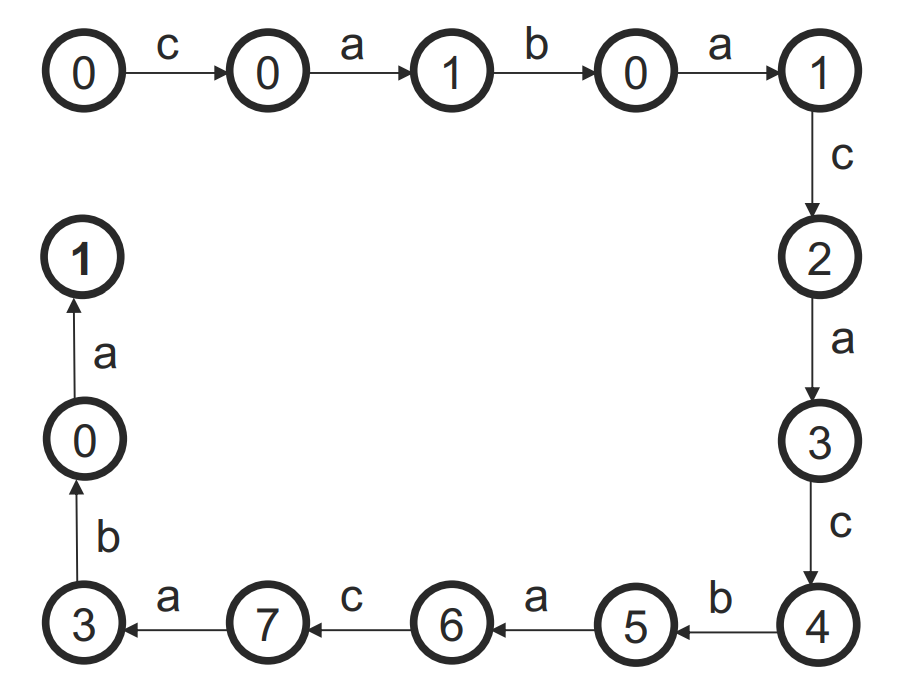
\includegraphics[width=0.3\textwidth]{img/pattern/ASF.png}
        \caption{Esecuzione dell'algoritmo per la ricerca esatta con Automa a
            Stati Finiti}
        \label{fig:enter-label}
    \end{figure}
\end{esempio}
\newpage
\section{Algoritmo di Knuth-Morris-Pratt}
Questo algoritmo per la ricerca esatta è basato su un'analisi del pattern. Si
hanno due fasi:
\begin{enumerate}
    \item \textbf{Preprocessing del pattern}: questa fase consiste nel calcolo
          della \textbf{prefix function} $\phi$, che è una funzione che associa
          ad ogni posizione del pattern la lunghezza del più lungo prefisso del
          pattern che è anche un suffisso del pattern. Questa funzione è calcolata
          in tempo lineare rispetto alla lunghezza del pattern $\mathcal{O}(m)$.
    \item \textbf{Scansione del testo}: questa fase consiste nel confrontare il
          pattern con il testo cercando di identificare le occorrenze esatte di
          esso. Questa fase è eseguita in tempo lineare rispetto alla lunghezza
          del testo $\mathcal{O}(n)$.
\end{enumerate}
La \textbf{prefix function} o funzione di fallimento $\phi$ è definita come segue:
\begin{equation}
    \phi: \{0, 1, \dots m\} \to \{-1, 0, \dots m\}
\end{equation}
Essa è definita come segue:
\begin{equation}
    \phi(j) = \begin{cases}
        |B(P[1, j])| & \text{se } 1 \leq j \leq m \\
        -1           & \text{se } j = 0
    \end{cases}
\end{equation}
\begin{esempio}
    Calcoliamo $\phi$ sul pattern $P=abcabaabcabab$ con $m=13$.
    \begin{table}[!ht]
        \centering
        \begin{tabular}{|>{\columncolor[HTML]{EFEFEF}}c|c|c|c|c|c|c|c|c|c|c|c|c|c|c|}\hline
            \cellcolor[HTML]{EFEFEF}\textbf{j}  &
            \cellcolor[HTML]{EFEFEF}\textbf{0}  &
            \cellcolor[HTML]{EFEFEF}\textbf{1}  &
            \cellcolor[HTML]{EFEFEF}\textbf{2}  &
            \cellcolor[HTML]{EFEFEF}\textbf{3}  &
            \cellcolor[HTML]{EFEFEF}\textbf{4}  &
            \cellcolor[HTML]{EFEFEF}\textbf{5}  &
            \cellcolor[HTML]{EFEFEF}\textbf{6}  &
            \cellcolor[HTML]{EFEFEF}\textbf{7}  &
            \cellcolor[HTML]{EFEFEF}\textbf{8}  &
            \cellcolor[HTML]{EFEFEF}\textbf{9}  &
            \cellcolor[HTML]{EFEFEF}\textbf{10} &
            \cellcolor[HTML]{EFEFEF}\textbf{11} &
            \cellcolor[HTML]{EFEFEF}\textbf{12} &
            \cellcolor[HTML]{EFEFEF}\textbf{13}                                  \\	\hline
            $\phi$                              & -1 & 0 & 0 & 0 & 1 & 2 & 1 & 1
                                                & 2  & 3 & 4 & 5 & 6 & 2         \\\hline
        \end{tabular}
    \end{table}
\end{esempio}
Questo algoritmo è un'evoluzione dell'algoritmo banale per la ricerca delle
occorrenze di un pattern in un testo. In particolare, l'algoritmo KMP consiste in:
\begin{enumerate}
    \item Viene usata una finestra $W$ di lunghezza $m$ che scorre sul testo $T$
          da sinistra a destra con posizione iniziale $i = 1$.
    \item Si confrontano i simboli di $P$ con i corrispondenti simboli di $T$
          all'interno della finestra $W$ andando da sinistra a destra e partendo
          dal primo simbolo di $P$.
    \item Non appena si incontra un \textit{mismatch} oppure ogni simbolo di $P$
          ha un match con il corrispondente simbolo in $W$ (i è occorrenza esatta),
          $W$ viene spostata a destra nella posizione:
          \begin{equation}
              p = i + j - \phi(j - 1) - 1
          \end{equation}
          dove $j$ è l'indice del simbolo di $P$ che ha causato il mismatch,
          mentre $i$ è la posizione iniziale di $W$.
    \item L'ultima posizione di $W$ è $n - m + 1$.
\end{enumerate}
Riassumendo:
\begin{itemize}
    \item $W$ viene spostata dalla posizione $i$ alla posizione $p$, dove:
          \begin{equation}
              p = i + j - \phi(j - 1) - 1
          \end{equation}
          con $j$ indice del simbolo di $P$ che ha causato il mismatch per $W$
          in posizione $i$.
    \item Il confronto riparte dal simbolo di $P$ in posizione $j = \phi(j - 1)
              + 1$ e dal simbolo di $T$ in posizione $i + j - 1$.
\end{itemize}
Nel caso in cui $j = 1$, allora $p = i + 1$ e il confronto riparte dal primo
simbolo di $P$ e dal simbolo di $T$ in posizione $i + 1$.
\begin{nota}
    Chiaramente il confronto riparte dalle posizioni $i + 1$ su $T$ e $1$ su P,
    ma dire che riparte dalla posizione $i$ su $T$ e dalla posizione $0$ su $P$
    implicitamente fa riferimento ad un confronto iniziale fittizio tra $T[i]$ e
    $P[0]$ (simbolo inesistente) che di default viene considerato un match.
\end{nota}
Nel caso in cui $j = m + 1$, allora $p = i + m - \phi(m)$ e il confronto
riparte dalla posizione $\phi(m) + 1$ di $P$ e dal simbolo di $T$ in posizione
$i + m$.
\begin{table}[!ht]
    \centering
    \begin{tabular}{|l|l|l|}
        \hline
                           & Automa a stati finiti     & KMP              \\ \hline
        Preprocessing di P & $\mathcal{O}(m |\Sigma|)$ & $\mathcal{O}(m)$ \\ \hline
        Scansione di T     & $\mathcal{O}(n)$          & $\mathcal{O}(n)$ \\ \hline
        Spazio             & $\mathcal{O}(m |\Sigma|)$ & $\mathcal{O}(m)$ \\ \hline
    \end{tabular}
\end{table}
Le differenze tra l'algoritmo basato sull'automa a stati finiti e KMP sono:
\begin{itemize}
    \item Automa:
          \begin{itemize}
              \item Efficiente per pattern piccoli, perché la memoria è contenuta
                    quindi le costanti all'interno del calcolo del tempo sono
                    migliori.
              \item Richiede più tempo e memoria per pattern grandi, perché
                    sprechiamo tempo nel calcolo del $\delta$.
              \item Ricerca di P in testi diversi utilizzando lo stesso automa.
          \end{itemize}
          KMP:
          \begin{itemize}
              \item Efficiente per pattern grandi.
              \item Richiede più tempo per pattern piccoli.
          \end{itemize}
\end{itemize}
\section{Algoritmo di Baeza-Yates e Gonnet}
La ricerca esatta effettuata attraverso questo algoritmo effettua un confronto
tra i simboli del pattern e del testo in maniera non esplicita, ovvero non
confronta carattere per carattere. In questo algoritmo vengono effettuate in
parallelo operazioni bit a bit su word di bit, viene anche chiamato
\textit{algoritmo bit parallel}.

Questo algoritmo segue il paradigma \textbf{shift-and} ovvero compie fondamentalmente
due sole operazioni:
\begin{itemize}
    \item \textbf{Shift} dei bit.
    \item \textbf{AND} logico tra i bit.
\end{itemize}
Come gli algoritmi visti fin ora, anche in questo caso possiamo descrivere il suo
funzionamento attraverso due fasi:
\begin{itemize}
    \item \textbf{Preprocessing del pattern} $P$ nel quale vengono calcolate
          $|\Sigma|$ \textbf{words} ognuna di $m$ bit. Questa operazione viene
          eseguita in tempo $\theta(m + |\Sigma|)$.
    \item \textbf{Scansione del testo} $T$ per cercare le occorrenze esatte del
          pattern $P$. Questa operazione viene eseguita in tempo $\theta(n)$.
\end{itemize}
\subsection{Word e Operatori}
\begin{definizione}[\textbf{Word di bit}]
    Una \textbf{word di bit} è un gruppo di bit che viene trattato come un'unità
    la cui dimensione può variare e che rappresenta un valore di un certo tipo,
    come ad esempio un numero o un carattere. In una word, il bit più a destra è
    quello meno significativo, mentre quello più a sinistra è quello più significativo.
\end{definizione}
Sulle word si possono eseguire delle operazioni \textit{bit a bit}, ovvero si
esegue un'operazione tra i bit corrispondenti di due o più words di bit della
stessa lunghezza. Il valore restituito da queste operazioni è una nuova word in
cui ogni bit è il risultato dell'operazione tra i bit corrispondenti nelle word
in input. Tra queste operazioni abbiamo:
\begin{itemize}
    \item \textbf{Congiunzione logica} $\to$ AND. Questa operazione è implementata
          come:
          \begin{equation}
              w = w_1 \ \text{AND} \ w_2
          \end{equation}
          restituisce una word $w$ tale che:
          \begin{equation}
              w[j] = \begin{cases}
                  1 & \text{se } w_1[j] = 1 \ \text{AND} \ w_2[j] = 1 \\
                  0 & \text{altrimenti}
              \end{cases}
          \end{equation}
    \item \textbf{Disgiunzione logica} (inclusiva) $\to$ OR. Questa operazione è
          implementata come:
          \begin{equation}
              w = w_1 \ \text{OR} \ w_2
          \end{equation}
          restituisce una word $w$ tale che:
          \begin{equation}
              w[j] = \begin{cases}
                  1 & \text{se } w_1[j] = 1 \ \text{OR} \ w_2[j] = 1 \\
                  0 & \text{altrimenti}
              \end{cases}
          \end{equation}
    \item \textbf{Shift dei bit} di una posizione a destra con bit più significativo
          a $0$ $\to$ RSHIFT. Questa operazione è implementata come:
          \begin{equation}
              w = \text{RSHIFT}(w_1)
          \end{equation}
          restituisce una word $w$ tale che:
          \begin{itemize}
              \item $w[j] = w_1[j - 1]$ se $j \geq 2$.
              \item $w[1] = 0$ altrimenti.
          \end{itemize}
    \item \textbf{Shift dei bit} di una posizione a destra con bit più significativo
          a $1$ $\to$ RSHIFT1. Questa operazione viene implementata come un RSHIFT
          seguito da un OR con una maschera in cui nella prima posizione è presente
          1 e nelle altre 0.
\end{itemize}
\subsection{Preprocessing del pattern}
Dato un pattern $P$ di lunghezza $m$ e $\sigma$ in $\Sigma$, $B_{\sigma}$ è una
word di $m$ bit tale che:
\begin{equation}
    B_{\sigma}[j] = 1 \iff P[j] = \sigma
\end{equation}
Viene creata una word per ogni simbolo dell'alfabeto $\Sigma$ e viene memorizzata
in una tabella $B$. Con questa rappresentazione posso effettuare le query del tipo:
\begin{center}
    Il simbolo in posizione $j$ di $P$ è uguale a un certo simbolo $\sigma$
\end{center}
\begin{esempio}
    Calcoliamo la tabella $B$ per un pattern $P=abcaba$ su un alfabeto $\Sigma =
        \{a, b, c, d\}$.
    \begin{table}[!ht]
        \centering
        \begin{tabular}{|c|c|c|c|c|c|c|}
            \hline
            P     & $a$ & $b$ & $c$ & $a$ & $b$ & $a$ \\ \hline
            $B_a$ & $1$ & $0$ & $0$ & $1$ & $0$ & $1$ \\ \hline
            $B_b$ & $0$ & $1$ & $0$ & $0$ & $1$ & $0$ \\ \hline
            $B_c$ & $0$ & $0$ & $1$ & $0$ & $0$ & $0$ \\ \hline
            $B_d$ & $0$ & $0$ & $0$ & $0$ & $0$ & $0$ \\ \hline
        \end{tabular}
    \end{table}
\end{esempio}
Vediamo ora come calcolare la tabella $B$:
\begin{enumerate}
    \item Tutte le word $B_{\sigma}$ vengono inizializzate a $m$ bit a $0$.
    \item Viene creata una maschera $M$ di $m$ bit tutti uguali a $0$ tranne il
          più significativo che è uguale a $1$.
    \item Si esegue una scansione di $P$ da sinistra a destra, e per ogni posizione
          $j$ vengono eseguite le due operazioni bit a bit:
          \begin{itemize}
              \item $B_{P[j]} = M \ \textbf{OR} \ B_{P[j]}$
              \item $M = \textbf{RSHIFT} (M)$
          \end{itemize}
\end{enumerate}
L'algoritmo per calcolare la tabella richiede un tempo pari a $\theta(|\Sigma| +
    m)$ ed è il seguente:
\begin{algorithm}
    \begin{algorithmic}
        \Function{Compute-table-B}{$P$}
        \State $m \gets |P|$
        \State $B \gets \text{empty table of} \ |\Sigma| \ \text{words} \ B_{\sigma}$
        \For{$\sigma \in \Sigma$}
        \State $B_{\sigma} \gets 00\dots0$
        \EndFor
        \State $M \gets 10\dots0$
        \For{$\sigma \in \Sigma$}
        \State $\sigma \gets P[j]$
        \State $B_{\sigma} \gets M \ \text{OR} \ B_{\sigma}$
        \State $M = \textbf{RSHIFT} (M)$
        \EndFor
        \State \textbf{return} $B$
        \EndFunction
    \end{algorithmic}
    \caption{Algoritmo per il calcolo della tabella $B$}
\end{algorithm}
\subsection{Scansione del testo}
La procedura per la scansione del testo è rappresentata come:
\begin{enumerate}
    \item Il testo $T$ viene scandito dalla prima all'ultima posizione.
    \item Per ogni posizione $i$ del testo $T$ viene calcolata una word $D_i$ di
          $m$ bit.
    \item Ogni volta che in $D_i$ il bit meno significativo è uguale a $1$, allora
          $i - m + 1$ è occorrenza esatta di $P$ in $T$.
\end{enumerate}
Dobbiamo ora definire cosa si intende con la word $D_i$. Prima di fare ciò dobbiamo
definire $P[1,j] = suff(T[1,i])$ ovvero $P[1,j]$ è uguale a un suffisso di $T[1,i]$.
\begin{definizione}[\textbf{Word $D_i$}]
    Dati un pattern $P$ lungo $m$ e un testo $T$ lungo $n$, $D_i$ ($0 \leq i \leq
        n$) è una word di $m$ bit tale che:
    \begin{equation}
        D_i[j] = 1 \iff P[1,j] = suff(T[1,i])
    \end{equation}
    Inoltre, sappiamo per definizione che:
    \begin{itemize}
        \item $D_0 = 00\dots0$ dato che $P[1, j] \neq suff(T[1, 0]) \ \forall j$
        \item $D_i[m] = 1$ se e solo se $P[1, m] = suff(T[1, i]) = T[i - m + 1,
                          i]$ ovvero si ha un'occorrenza esatta di $P$ in $T$
              nella posizione $i - m + 1$.
    \end{itemize}
\end{definizione}
\begin{nota}
    Nota che da $D_i$ possiamo anche ottenere la lunghezza del bordo del pattern.
    In generale, data una word $D_i$, la lunghezza del bordo del pattern $P$ è
    uguale a $j$ se e solo se $D_i[m] = 1$ e $j$ è la più grande posizione $< m$
    tale che $D_i[j] = 1$.

    Con posizione più grande si intende quella più a destra diversa da $m$.
\end{nota}
\begin{esempio}
    Data la word:
    \begin{table}[!ht]
        \centering
        \begin{tabular}{|c|c|c|c|c|c|c|c|c|c|c|c|c|c|c|c|c|}
            D\_i & 0 & 1 & 1 & 0 & 0 & 0 & 1 & 1 & 0 & 0  & 1  & 0  & 0  & 0  & 0  & 1  \\ \hline
            ~    & 1 & 2 & 3 & 4 & 5 & 6 & 7 & 8 & 9 & 10 & 11 & 12 & 13 & 14 & 15 & 16 \\
        \end{tabular}
    \end{table}
    possiamo calcolare il bordo del pattern in quanto l'ultimo bit è uguale a $1$.
    Dato che il bit con valore uguale a $1$ più a destra, diverso da $m$, è in
    posizione $11$, allora la lunghezza del bordo è:
    \begin{equation}
        |B(P)| = 11
    \end{equation}
\end{esempio}
Ovviamente calcolare $D_i$ è sempre troppo costoso, infatti, $D_i$ viene sempre
ottenuto a partire da $D_{i - 1}$, portando a modificare l'algoritmo di scansione
del testo nel seguente modo:
\begin{itemize}
    \item Inizia dalla word $D_0 = 00\dots0$
    \item Per ogni $i$ da $1$ a $n$ calcola la word $D_i$ a partire dalla word
          $D_{i - 1}$.
    \item Ogni volta che $D_i$ ha il bit meno significativo uguale a $1$, viene
          prodotta in output l'occorrenza $i - m + 1$.
\end{itemize}
Vediamo ora come si calcola il valore di $D_i$ a partire da $D_{i - 1}$:
\begin{itemize}
    \item Se $j =  1$ allora posso calcolarla come:
          \begin{equation}
              D_i[1] = 1 \textbf{AND} B_{T[i]}[1]
          \end{equation}
          Perché $D_i[1] = 1 \iff P[1,1] = suff(T[1,i]) \iff P[1] = T[i] \iff
              B_{T[i]}[1]$. Si aggiunge $1$ per semplificare le operazioni bit
          a bit.
    \item Se $j > 1$ allora posso calcolarla come:
          \begin{equation}
              D_i[j] = D_{i - 1}[j - 1] \textbf{AND} B_{T[i]}[j]
          \end{equation}
          Perché $D_i[j] = 1 \iff P[1,j] = suff(T[1,i]) \iff P[1,j - 1] =
              suff(T[1,i - 1]) \textbf{AND} P[j] = T[i] \iff D_{i - 1}[j - 1]
              \textbf{AND} B_{T[i]}[j]$.
\end{itemize}
In questo modo stiamo ancora aggiornando un bit alla volta, ma sfruttando le
operazioni bit a bit si possono aggiornare tutti in tempo \textbf{costante} nel
seguente modo:
\begin{equation}
    D_i = \textbf{RSHIFT1}(D_{i - 1}) \ \textbf{AND} \ B_{T[i]}
\end{equation}
Vediamo ora come implementare l'algoritmo che effettua la scansione del testo in
tempo $\theta(n)$
\begin{algorithm}
    \begin{algorithmic}
        \Function{BYG}{$B, T$}
        \State $n \gets |T|$
        \State $D \gets 00\dots0$
        \State $M \gets 00\dots01$
        \For{$i \gets 1 \ \text{to} \ n$}
        \State $\sigma \gets T[i]$
        \State $D \gets \textbf{RSHIFT1}(D_{i - 1}) \ \textbf{AND} \ B_{T[i]}$
        \If{$(D \ \textbf{AND} M) = M$}
        \State \text{output} $i - m + 1$
        \EndIf
        \EndFor
        \EndFunction
    \end{algorithmic}
    \caption{Algoritmo per la scansione del testo}
\end{algorithm}
\begin{esempio}
    Siano un testo $T = babcabaadc$ e un pattern $P = abcaba$ tale che $|T| = 10$
    e $|P|=6$. Entrambe le stringhe costruite su un alfabeto $\Sigma = \{a, b, c,
        d\}$, allora costruiamo la tabella $B_\sigma$:
    \begin{table}[!ht]
        \centering
        \begin{tabular}{|c|c|c|c|c|c|c|}
            \hline
            P     & $a$ & $b$ & $c$ & $a$ & $b$ & $a$ \\ \hline
            $B_a$ & $1$ & $0$ & $0$ & $1$ & $0$ & $1$ \\ \hline
            $B_b$ & $0$ & $1$ & $0$ & $0$ & $1$ & $0$ \\ \hline
            $B_c$ & $0$ & $0$ & $1$ & $0$ & $0$ & $0$ \\ \hline
            $B_d$ & $0$ & $0$ & $0$ & $0$ & $0$ & $0$ \\ \hline
        \end{tabular}
    \end{table}
    I singoli passi sono i seguenti:
    \begin{itemize}
        \item Quindi partiremo da $D_0 = 000000$, leggo il primo simbolo del
              testo $T[1] = b$ e poi calcolo:
              \begin{equation}
                  D_1=RSHIFT1(D_{0}) \text{ AND } B_b = 100000 \text{ AND }
                  010010 = 000000
              \end{equation}
        \item Leggo il secondo simbolo del testo $T[2] = a$ e poi calcolo $D_2$:
              \begin{equation}
                  D_2 = 100000 \text{ AND } 100101 = 100000
              \end{equation}
        \item Leggo il secondo simbolo del testo $T[3] = b$ e poi calcolo $D_3$:
              \begin{equation}
                  D_3 = 110000 \text{ AND } 010010 = 010000
              \end{equation}
        \item Leggo il secondo simbolo del testo $T[4] = c$ e poi calcolo $D_4$:
              \begin{equation}
                  D_4 = 101100 \text{ AND } 001000 = 001000
              \end{equation}
        \item Leggo il secondo simbolo del testo $T[5] = a$ e poi calcolo $D_5$:
              \begin{equation}
                  D_5 = 100100 \text{ AND } 100101 = 100100
              \end{equation}
        \item $\dots$
        \item Leggo il secondo simbolo del testo $T[7] = a$ e poi calcolo $D_7$
              \begin{equation}
                  D_6 = 101001 \text{ AND } 100101 = 100001
              \end{equation}
        \item Ho il bit LSB di $D_6$ uguale a $1$, quindi ho trovato un match che
              corrisponde a $i - m + 1 = 7 - 6 + 1 = 2$. Poi continuo fino a
              quando non termino $T$.
    \end{itemize}
\end{esempio}
\section{Algoritmo di Wu e Manber}
L'algoritmo risolvere problemi di \textbf{string matching approssimati} e il
funzionamento è simile all'algoritmo \textbf{BYG}.
Riprendiamo la definizione di ricerca approssimata di un pattern $P$ in un testo
$T$:
\begin{definizione}[\textbf{Occorrenza approssimata}]
    Una posizione $i$ del testo $T$ tale che esista una sottostringa $S = T[i -
                L + 1]$ tale che $ED(P, S) \leq k$ è detta \textbf{occorrenza
        approssimata} di $P$ in $T$.
\end{definizione}
Come gli algoritmi visti fino a questo momento, quello di Wu e Manber è
strutturato in due fasi:
\begin{enumerate}
    \item \textbf{Preprocessing} del pattern $P$ nel quale vengono calcolate
          $|\Sigma|$ \textbf{words} ognuna di $m$ bit. Questa operazione viene
          eseguita in tempo $\Theta(|\Sigma| + m)$. (\textit{Uguale a quello
              dell'algoritmo BYG})
    \item \textbf{Scansione del testo} $T$ per cercare le occorrenze approssimate
          del pattern $P$. Questa operazione viene eseguita in tempo
          $\Theta(k \cdot n)$.
\end{enumerate}
\subsection{Scansione del testo}
Dato che la fase di preprocessing è equivalente a quella per l'algoritmo BYG,
passiamo subito alla scansione del testo.
\begin{definizione}
    Definiamo $P[1, j] = suff_h(T[1, i])$ ovvero $P[1, j]$ è uguale a un
    suffisso di $T[1, i]$ a meno di $h$ errori. In altre parole, riesco a
    trovare un suffisso $S$ di $T[1, i]$ tale che $ED(P[1, j], S) \leq h$.
\end{definizione}
Estenderemo la definizione di $D_i$ di Shift-AND al caso in cui si ammettono al
più $h$ errori.
\begin{definizione}[\textbf{Word $D_i^h$}]
    Dati un pattern $P$ lungo $m$, un testo $T$ lungo $n$ e una soglia di errore
    $k$, possiamo definire la \textbf{word $D_i^h$} come una word di $m$ bit
    tale che:
    \begin{equation}
        D_i^h[j] = 1 \iff P[1, j] = suff_h(T[1, i])
    \end{equation}
\end{definizione}
Vediamo ora alcuni casi particolare:
\begin{itemize}
    \item $D_i^0$: ovvero la la word con $h = 0$, è per definizione la word
          $D_i$ dell'algoritmo BYG.
    \item $D_0^h$: ovvero la word con $i = 0$, è tale che:
          \begin{itemize}
              \item $j \leq h \implies D_0^h[j] = 1$, questo perché $P[1, j]$ è
                    un prefisso di $T[1, 0]$ e quindi $ED(P[1, j], T[1, 0])
                        \leq h$.
              \item $j > h \implies D_0^h[j] = 0$, questo perché $P[1, j]$ non
                    è un prefisso di $T[1, 0]$ e quindi $ED(P[1, j], T[1, 0]) >
                        h$.
          \end{itemize}
          Si ottiene quindi una word dove i primi $h$ bit sono uguali a $1$ e i
          restanti $m - h$ bit sono posti a $0$.
    \item $D_i^h [m] = 1 \iff P[1, m] = suff_h(T[1, i])$, ovvero se $P[1, m]$ è
          un suffisso di $T[1, i]$ a meno di $h$ errori, allora $D_i^h[m] = 1$.
          Nel caso particolare in cui $h = 0$ si ha un occorrenza esatta in $i -
              m + 1$. Mentre nel caso in cui $h = k$ si ha un'occorrenza
          approssimata in posizione $i$.
\end{itemize}
\begin{nota}
    In generale, $D_i^{h'}[j] = 1$ implica $D_i^{h}[j] = 1$ con $h > h'$.
    Inoltre, $D_{i}^{h} [j] = 1$ implica $D_{i}^{h + 1}[j + 1] = 1$ e
    $D_{i}^{h + 1}[j - 1] = 1$.
\end{nota}
Definita la word $D_i^h$, possiamo definire la scansione del testo $T$ come una
successione di $k + 1$ scansioni, dove solamente all'iterazione $k$ si vanno a
verificare i bit finali delle word per cercare l'occorrenza approssimata.
Nello specifico, se all'iterazione $k$ si ha che $D_i^k[m] = 1$, allora si ha in
output l'occorrenza approssimata $i$.

Fino ad ora abbiamo definito come calcolare il caso in cui $h = 0$ oppure il
caso in cui $i = 0$. Vediamo ora come calcolare il caso in cui $i > 0, h > 0$:
\begin{itemize}
    \item $j > 1$: in questa situazione possiamo distinguere i seguenti casi:
          \begin{itemize}
              \item Si ha un \textbf{match} tra $P[j]$ e $T[i]$ \textbf{senza
                        errori}:
                    \begin{equation}
                        D_i^h[j] = 1 \iff P[1, j] = suff_h(T[1, i]) \Leftarrow
                        P[1, j - 1] = suff_h(T[1, i - 1]) \  \textbf{AND} \ T[i]
                        = P[j]
                    \end{equation}
                    ovvero $D_i^h[j] = 1$ se e solo se $P[1, j - 1]$ è un
                    suffisso di $T[1, i - 1]$ a meno di $h$ errori e $T[i] =
                        P[j]$. Questo significa che $D_i^h[j] = 1$ se e solo se:
                    \begin{equation}
                        D_{i - 1}^h[j - 1] = D_{i - 1}^h [j - 1] = 1 \
                        \textbf{AND} \ B_{T[i]} [j] =  1
                    \end{equation}
              \item \textbf{Non si ha un match} tra $P[j]$ e $T[i]$,
                    quindi si effettua un'\textbf{operazione di sostituzione}.
                    \begin{equation}
                        D_i^h[j] = 1 \iff P[1, j] = suff_h(T[1, i]) \Leftarrow
                        P[1, j - 1] = suff_{h - 1}(T[1, i - 1])
                    \end{equation}
                    ovvero non ho ancora raggiunto il limite di errori e quindi
                    posso ancora avere errori senza superare la soglia $h$.
                    Questo significa che $D_i^h[j] = 1$ se e solo se:
                    \begin{equation}
                        D_i^h[j] = 1 \Leftarrow D_{i - 1}^{h - 1} [j - 1] = 1
                    \end{equation}
              \item \textbf{Non si ha un match} tra $P[j]$ e $T[i]$, quindi si
                    effettua un'\textbf{operazione di inserimento} in $T$.
                    \begin{equation}
                        D_i^h[j] = 1 \iff P[1, j] = suff_h(T[1, i]) \Leftarrow
                        P[1, j] = suff_{h - 1}(T[1, i - 1])
                    \end{equation}
                    ovvero non ho ancora raggiunto il limite di errori. Questo
                    significa che $D_i^h[j] = 1$ se e solo se:
                    \begin{equation}
                        D_i^h[j] = 1 \Leftarrow D_{i - 1}^{h - 1} [j] = 1
                    \end{equation}
              \item \textbf{Non si ha un match} tra $P[j]$ e $T[i]$, quindi si
                    effettua un'\textbf{operazione di inserimento} in $P$.
                    \begin{equation}
                        D_i^h[j] = 1 \iff P[1, j] = suff_h(T[1, i]) \Leftarrow
                        P[1, j - 1] = suff_{h - 1}(T[1, i])
                    \end{equation}
                    ovvero non ho ancora raggiunto il limite di errori. Questo
                    significa che $D_i^h[j] = 1$ se e solo se:
                    \begin{equation}
                        D_i^h[j] = 1 \Leftarrow D_{i}^{h - 1} [j - 1] = 1
                    \end{equation}
          \end{itemize}
          A questo punto posso riassumere queste casistiche in un'unica formula:
          \begin{equation}
              D_{i}^{h} [j] =
              (D_{i - 1}^{h} [j - 1] \ \textbf{AND} \ B_{T[i]} [j]) \ \textbf{OR}
              \ D_{i - 1}^{h - 1} [j - 1] \ \textbf{OR}
              \ D_{i - 1}^{h - 1} [j] \ \textbf{OR}
              \ D_{i}^{h - 1} [j - 1]
          \end{equation}
    \item  $j = 1$, abbiamo le stesse casistiche di prima, quindi possiamo
          sostituire alla formula precedente il valore di $j$, comportando che
          ci richiedono dei valori che non possiamo conoscere come
          $D_{i - 1}^h[0]$. Quindi, per risolvere questo problema, sostituiamo
          questi valori con $1$, ottenendo:
          \begin{equation}
              D_{i}^{h} [j] =
              (1 \ \textbf{AND} \ B_{T[i]} [j]) \ \textbf{OR}
              \ 1 \ \textbf{OR}
              \ D_{i - 1}^{h - 1} [j] \ \textbf{OR}
              \ 1
          \end{equation}
\end{itemize}
Si possono unire i due macro casi sopracitati, sostituendo tutte le operazioni
che controllano il bit in posizione $j - 1$ con l'operazione RSHIFT1, ottenendo:
\begin{equation}
    D_{i}^{h} [j] =
    (RSHIFT1(D_{i - 1}^{h} [j]) \ \textbf{AND} \ B_{T[i]} [j]) \ \textbf{OR} \
    RSHIFT1(D_{i - 1}^{h - 1} [j]) \ \textbf{OR} \
    D_{i - 1}^{h - 1} [j] \ \textbf{OR} \
    RSHIFT1(D_{i}^{h - 1} [j])
\end{equation}
Si potrà poi generalizzare calcolando $D_i^h$ in una sola volta.
\begin{equation}
    D_{i}^{h}= (RSHIFT1(D_{i - 1}^{h}) \ \textbf{AND} \ B_{T[i]}) \
    \textbf{OR} \ RSHIFT1(D_{i - 1}^{h - 1})  \ \textbf{OR} \ D_{i - 1}^{h - 1} \
    \textbf{OR} \ RSHIFT1(D_{i}^{h - 1})
\end{equation}
Vediamo ora come è possibile implementare l'algoritmo per la scansione del testo:
\begin{enumerate}
    \item Inizializzazione della parola $D_0^0$ a $00\dots0$.
    \item Calcolo di $D_i^0$ per $i = 1, \dots, n$, utilizzando l'algoritmo di
          BYG.
    \item Per $h$ da $1$ a $k$:
          \begin{enumerate}
              \item Calcolo di $D_0^h$.
              \item Per $i$ da $1$ a $n$:
                    \begin{enumerate}
                        \item Calcolo di $D_i^h$ a partire da $D_{i - 1}^h$.
                        \item Se $D_i^h[m] = 1 \ \textbf{AND} \ h = k$ allora
                              output $i$.
                    \end{enumerate}
          \end{enumerate}
\end{enumerate}
\section{Strutture di indicizzazione del testo}
Per rendere più efficiente la ricerca di un pattern esatto si effettuano delle
operazioni di preprocessing del testo che permettono di ristrutturarlo per
accedere velocemente alle sue porzioni.

Le strutture di indicizzazione sono strutture che manipolano l'input in modo da
rendere più efficiente le operazioni su di esso, ma hanno il problema che
richiedono molta memoria. Inoltre, la loro costruzione risulta complessa.

Queste strutture si basano su:
\begin{itemize}
    \item \textbf{Ordine lessicografico}: si definisce un ordine lessicografico
          dei caratteri dell'alfabeto per poter determinare un ordine delle
          parole.
    \item \textbf{Carattere terminatore} $\$$: è il carattere più piccolo
          dell'alfabeto che serve per identificare il termine della stringa.
\end{itemize}
In aggiunta dovremo definire:
\begin{definizione}[\textbf{q-suffisso}]
    Il suffisso di indice $q$ ($q$-suffisso) è il suffisso che inizia nella
    posizione $q$ del testo, quindi $T[q:]= T[q:|T|]$.
\end{definizione}
Il suffisso del carattere terminatore è il carattere terminatore stesso.
\begin{definizione}[\textbf{Ordinamento dei suffissi}]
    Definiremo l'ordinamento dei suffissi nel segunete modo. Dati due suffissi
    $s$ e $s'$, sia $i$ la più piccola posizione tale che $s[i] \neq s'[i]$, dove:
    \begin{itemize}
        \item $s \prec s'\iff s[i] < s'[i]$
        \item $s \succ s'\iff s[i] > s'[i]$
    \end{itemize}
\end{definizione}
\subsection{Suffix Array}
Questa struttura di indicizzazione è stata inventata da Myers e Manber nel 1990,
non contiene l'informazione sui simboli del testo e occupa $\Theta(n \log n)$ 
spazio (contando i bit per rappresentare le posizioni intere). 
Questa struttura permette di effettuare la ricerca esatta di un pattern
$P$ su  un testo $T$ in tempo $\mathcal{O}(|P| \log |T|)$.
\begin{definizione}[\textbf{Suffix Array}]
    Il \textbf{suffix array} di un testo $T$ lungo $n$ è un array $S$ lungo $n$,
    tale che $S[i]= q$ se e solo se il $q$-suffisso è l'$i$-esimo suffisso
    nell'ordinamento lessicografico dei suffissi di $T$.
\end{definizione}
\begin{esempio}
    Consideriamo il testo $T = ggtcagtc\$$, il cui ordinamento lessicografico è
    definito come:
    \begin{equation}
        \$ < a < c < g < t
    \end{equation}
    Possiamo costruire il suffix array $S$ nel seguente modo:
    \begin{itemize}
        \item Generiamo tutti i suffissi di $T$:
              \begin{table}[!ht]
                  \centering
                  \begin{tabular}{|
                          >{\columncolor[HTML]{EFEFEF}}l|lllllllll|}
                      \hline
                      \textbf{SA}                        &
                      \cellcolor[HTML]{EFEFEF}\textbf{1} &
                      \cellcolor[HTML]{EFEFEF}\textbf{2} &
                      \cellcolor[HTML]{EFEFEF}\textbf{3} &
                      \cellcolor[HTML]{EFEFEF}\textbf{4} &
                      \cellcolor[HTML]{EFEFEF}\textbf{5} &
                      \cellcolor[HTML]{EFEFEF}\textbf{6} &
                      \cellcolor[HTML]{EFEFEF}\textbf{7} &
                      \cellcolor[HTML]{EFEFEF}\textbf{8} &
                      \cellcolor[HTML]{EFEFEF}\textbf{9}                                              \\ \hline
                      \textbf{1}                         & g  & g  & t  & c  & a  & g  & t  & c  & \$ \\ \hline
                      \textbf{2}                         & g  & t  & c  & a  & g  & t  & c  & \$ &    \\ \hline
                      \textbf{3}                         & t  & c  & a  & g  & t  & c  & \$ &    &    \\ \hline
                      \textbf{4}                         & c  & a  & g  & t  & c  & \$ &    &    &    \\ \hline
                      \textbf{5}                         & a  & g  & t  & c  & \$ &    &    &    &    \\ \hline
                      \textbf{6}                         & g  & t  & c  & \$ &    &    &    &    &    \\ \hline
                      \textbf{7}                         & t  & c  & \$ &    &    &    &    &    &    \\ \hline
                      \textbf{8}                         & c  & \$ &    &    &    &    &    &    &    \\ \hline
                      \textbf{9}                         & \$ &    &    &    &    &    &    &    &    \\ \hline
                  \end{tabular}
              \end{table}
        \item Ordiniamo i suffissi in ordine lessicografico:
              \begin{table}[!ht]
                  \centering
                  \begin{tabular}{|
                          >{\columncolor[HTML]{EFEFEF}}l |lllllllll|}
                      \hline
                      \textbf{SA}                        &
                      \cellcolor[HTML]{EFEFEF}\textbf{1} &
                      \cellcolor[HTML]{EFEFEF}\textbf{2} &
                      \cellcolor[HTML]{EFEFEF}\textbf{3} &
                      \cellcolor[HTML]{EFEFEF}\textbf{4} &
                      \cellcolor[HTML]{EFEFEF}\textbf{5} &
                      \cellcolor[HTML]{EFEFEF}\textbf{6} &
                      \cellcolor[HTML]{EFEFEF}\textbf{7} &
                      \cellcolor[HTML]{EFEFEF}\textbf{8} &
                      \cellcolor[HTML]{EFEFEF}\textbf{9}                                              \\ \hline
                      \textbf{9}                         & \$ &    &    &    &    &    &    &    &    \\ \hline
                      \textbf{5}                         & a  & g  & t  & c  & \$ &    &    &    &    \\ \hline
                      \textbf{8}                         & c  & \$ &    &    &    &    &    &    &    \\ \hline
                      \textbf{4}                         & c  & a  & g  & t  & c  & \$ &    &    &    \\ \hline
                      \textbf{1}                         & g  & g  & t  & c  & a  & g  & t  & c  & \$ \\ \hline
                      \textbf{6}                         & g  & t  & c  & \$ &    &    &    &    &    \\ \hline
                      \textbf{2}                         & g  & t  & c  & a  & g  & t  & c  & \$ &    \\ \hline
                      \textbf{7}                         & t  & c  & \$ &    &    &    &    &    &    \\ \hline
                      \textbf{3}                         & t  & c  & a  & g  & t  & c  & \$ &    &    \\ \hline
                  \end{tabular}
              \end{table}
        \item Otteniamo il suffix array $S$ prendendo la colonna contenete gli
              indici dei suffissi: $S = [9, 5, 8, 4, 1, 6, 2, 7, 3]$
    \end{itemize}
\end{esempio}
Possiamo interpretare il suffix array come un array di indici, dove ogni elemento
$S[i]$ rappresenta la posizione del suffisso $i$-esimo nell'ordinamento.

Lo spazio richiesto per la memorizzazione del suffix array è $\Theta(n \log n)$.
\subsubsection{Ricerca esatta}
Vediamo ora il funzionamento della ricerca esatta di un pattern $P$ di lunghezza
$m$ in testo $T$ di lunghezza $n$.

La ricerca esatta di un pattern $P$ in un testo $T$ avviene in due fasi:
\begin{enumerate}
    \item Preprocessing del testo $T$ per costruire il suffix array $S$.
    \item Ricerca del pattern $P$ nel testo $T$ utilizzando il suffix array $S$.
          L'operazione di ricerca avviene in tempo $\Theta(m \log n)$.
\end{enumerate}
Per prima cosa si può osservare che:
\begin{itemize}
    \item Se $P$ occorre $k$ volte in $T$ allora $P$ è prefisso di $k$ suffissi
          di $T$. Ad esempio, dato il testo $T = xabxab\$$ e il pattern $P = ab$,
          possiamo osservare che $P$ occorre $2$ volte in $T$ il che implica che
          $P$ è prefisso di due suffissi di $T$, ovvero $2$-suffisso e
          $5$-suffisso.
    \item Gli indici dei $k$ suffissi sono le occorrenze di $P$ e sono consecutivi
          nel suffix array. Ad esempio, dato il testo $T = xabxab\$$ possiamo
          calcolare il suo suffix array e ottenere $S=[7, 5, 2, 6, 3, 4, 1]$. Se
          consideriamo il pattern $P = ab$ possiamo osservare che  esso occorre
          $2$ volte in $T$ nelle posizioni $2$ e $5$ che sono consecutive.
    \item Se $P$ occorre in posizione $q$ di $T$ ed è lessicograficamente minore
          (maggiore) del suffisso di indice $q'$, allora anche il suffisso di
          indice $q$ (che contiene $P$ come prefisso) è lessicograficamente
          minore (maggiore) del suffisso di indice $q'$.
\end{itemize}
Quindi l'algortmo di ricerca sarà:
\begin{enumerate}
    \item Si inizializza un intervallo di posizioni $[L,R] = [1, |T|]$.
    \item \label{passo-2-sa} Si considera il suffisso di indice $S[p]$ con
          $p = \left\lfloor \frac{R - L}{2} \right\rfloor$, e in tempo $O(m)$ si
          controlla:
          \begin{itemize}
              \item $P \prec S[p]$-suffisso: si ripete il punto \ref{passo-2-sa}
                    ponendo $[L, R] = [L, p]$.
              \item $P \succ S[p]$-suffisso: si ripete il punto \ref{passo-2-sa}
                    ponendo $[L, R] = [p + 1, R]$.
              \item $P$ occorre come prefisso in $S[p]$-suffisso: si termina e
                    si restituisce la posizione $S[p]$.
          \end{itemize}
\end{enumerate}
Questo algoritmo trova un'occorrenza del pattern $P$ in tempo $O(|P| \log |T|)$.
Nel caso in cui si desidera ottenere tutte le occorrenze di $P$ in $T$ è
necessario modificarlo.
\begin{algorithm}[!ht]
    \begin{algorithmic}
        \Function{SuffixArraySearch}{$T, P$}
        \State $n \gets |T|$
        \State $m \gets |P|$
        \State $S \gets$ \Call{SuffixArray}{$T$}
        \State $l \gets 1$
        \State $r \gets n$
        \While{$l \leq r$}
        \State $p \gets \lfloor (l + r) / 2 \rfloor$
        \If{$P < S[p]-$suffisso}
        \State $r \gets p - 1$
        \ElsIf{$P > S[p]-$suffisso}
        \State $l \gets p + 1$
        \Else
        \State \Return $p$
        \EndIf
        \EndWhile
        \State \Return $-1$
        \EndFunction
    \end{algorithmic}
    \caption{Algoritmo di ricerca esatta di un pattern}
\end{algorithm}
\subsection{Burrows Wheeler Transform}
Proposta da Burrows e Wheeler nel '94, costruisce una permutazione reversibile
dei simboli del testo, occupa uno spazio di $\Theta(|T| \log |\Sigma|)$ ed è
usata in B-zip 2.

Prima di definire la trasformata di Burrows-Wheeler, definiamo il concetto di
\textbf{rotazione di indice $q$}.
\begin{definizione}[\textbf{q-rotazione}]
    La rotazione di indice $q$ ($q$-rotazione) è la concatenazione del
    $q$-suffisso $T[q, |T|]$ e del prefisso $T[1, q - 1]$.
    \begin{equation}
        r_q = T[q, |T|] \cdot T[1, q - 1]
    \end{equation}
\end{definizione}
\begin{esempio}
    Dato il seguente testo $T = ggtcagtc\$$, allora possiamo calcolare:
    \begin{itemize}
        \item La $3$-rotazione come: $$tcagtc\$gg$$
        \item La $9$-rotazione come: $$\$ggtcagtc$$
        \item La $1$-rotazione come: $$ggtcagtc\$$$
    \end{itemize}
\end{esempio}
Possiamo osservare che la $q$-rotazione $r$ è una stringa lunga $n$ che ha:
\begin{enumerate}
    \item Il $q$-suffisso come prefisso.
    \item Il prefisso lungo $q - 1$ come suffisso.
\end{enumerate}
Questo significa che per la rotazione $q$-rotazione denominata $r$:
\begin{itemize}
    \item $r[1]$ è uguale a $T[q]$ (primo simbolo del $q$-suffisso).
    \item $r[n]$ è uguale a $T[q - 1]$ se $q > 1$, questo implica che:
          \begin{itemize}
              \item L'ultimo simbolo della $q$-rotazione è il simbolo iniziale
                    della $q - 1$-rotazione.
              \item Il $q - 1$-suffisso contiene il $q$-suffisso come suffisso
                    se $q > 1$.
          \end{itemize}
    \item $r[n]$ è uguale a $T[n]$ se $q = 1$, questo implica che:
          \begin{itemize}
              \item L'ultimo simbolo della $q$-rotazione è il simbolo iniziale
                    della $n$-rotazione (e quindi dell'$n$-suffisso)
          \end{itemize}
\end{itemize}
Definiremo anche una regola di ordinamento:
\begin{definizione}[\textbf{Ordinamento delle rotazioni}]
    Date due rotazioni $r$ e $r'$, sia $i$ la più piccola posizione tale che
    $r[i]\ne r'[i]$, dove:
    \begin{itemize}
        \item $r \prec r'\iff r[i] < r'[i]$
        \item $r \succ r'\iff r[i] > r'[i]$
    \end{itemize}
\end{definizione}
Possiamo introdurre questi teoremi:
\begin{teorema}
    \label{th:ord-rot-1}
    Sia $q$-rotazione $r_1$ una $p$-rotazione $r_2$ tale che:
    \begin{itemize}
        \item $r_1 \prec r_2$
        \item $r_1[n] = r_2[n]$
    \end{itemize}
    Allora $(q - 1)$-rotazione $r'_1$ è minore della $(p - 1)$-rotazione $r'_2$.
\end{teorema}
\begin{teorema}
    \label{th:ord-rot-2}
    Sia $q$-rotazione $r_1$ una $p$-rotazione $r_2$ tale che $r_1[n] \prec r_2[n]$,
    Allora $(q - 1)$-rotazione $r'_1$ è minore della $(p - 1)$-rotazione $r'_2$.
\end{teorema}
Dopo questo preambolo si può definire la trasformata di Burrows-Wheeler:
\begin{definizione}[\textbf{Burrows Wheeler Transform}]
    La $BWT$ $B$ di un testo $T$ lungo $n$ è un array di lunghezza $n$ tale che
    $B[i] = r_i[n]$ se e solo se $r_i$ è l'$i$-esima rotazione nell'ordinamento
    lessicografico delle rotazioni di $T$.

    In altri termini, $B[i]$ è l'ultimo simbolo della rotazione $r_i$ che è
    l'$i$-esima rotazione nell'ordinamento lessicografico e che sarà la
    $q$-rotazione per un certo valore $q$.
\end{definizione}
Ecco un esempio di costruzione:
\begin{esempio}
    Consideriamo il testo $T = ggtcagtc\$$, il cui ordinamento lessicografico è
    definito come:
    \begin{equation}
        \$ < a < c < g < t
    \end{equation}
    Possiamo costruire la Burrows Wheeler Transform $BWT$ nel seguente modo:
    \begin{itemize}
        \item Elenchiamo tutte le rotazioni del testo \ref{tab:rotazioni}:
              \begin{table}[!ht]
                  \centering
                  \begin{tabular}{|
                          >{\columncolor[HTML]{EFEFEF}}l |lllllllll|}
                      \hline
                      \textbf{BWT}                       &
                      \cellcolor[HTML]{EFEFEF}\textbf{1} &
                      \cellcolor[HTML]{EFEFEF}\textbf{2} &
                      \cellcolor[HTML]{EFEFEF}\textbf{3} &
                      \cellcolor[HTML]{EFEFEF}\textbf{4} &
                      \cellcolor[HTML]{EFEFEF}\textbf{5} &
                      \cellcolor[HTML]{EFEFEF}\textbf{6} &
                      \cellcolor[HTML]{EFEFEF}\textbf{7} &
                      \cellcolor[HTML]{EFEFEF}\textbf{8} &
                      \cellcolor[HTML]{EFEFEF}\textbf{9}                                              \\ \hline
                      \textbf{1}                         & g  & g  & t  & c  & a  & g  & t  & c  & \$ \\ \hline
                      \textbf{2}                         & g  & t  & c  & a  & g  & t  & c  & \$ & g  \\ \hline
                      \textbf{3}                         & t  & c  & a  & g  & t  & c  & \$ & g  & g  \\ \hline
                      \textbf{4}                         & c  & a  & g  & t  & c  & \$ & g  & g  & t  \\ \hline
                      \textbf{5}                         & a  & g  & t  & c  & \$ & g  & g  & t  & c  \\ \hline
                      \textbf{6}                         & g  & t  & c  & \$ & g  & g  & t  & c  & a  \\ \hline
                      \textbf{7}                         & t  & c  & \$ & g  & g  & t  & c  & a  & g  \\ \hline
                      \textbf{8}                         & c  & \$ & g  & g  & t  & c  & a  & g  & t  \\ \hline
                      \textbf{9}                         & \$ & g  & g  & t  & c  & a  & g  & t  & c  \\ \hline
                  \end{tabular}
                  \caption{Rotazioni del testo}
                  \label{tab:rotazioni}
              \end{table}
        \item Ordiniamo le rotazioni secondo l'ordine lessicografico \ref{tab:rotazioni-ord}:
              \begin{table}[!ht]
                  \centering
                  \begin{tabular}{|
                          >{\columncolor[HTML]{EFEFEF}}l |l|l|l|l|l|l|l|l|l|}
                      \hline
                      \textbf{BWT}                       &
                      \cellcolor[HTML]{EFEFEF}\textbf{1} &
                      \cellcolor[HTML]{EFEFEF}\textbf{2} &
                      \cellcolor[HTML]{EFEFEF}\textbf{3} &
                      \cellcolor[HTML]{EFEFEF}\textbf{4} &
                      \cellcolor[HTML]{EFEFEF}\textbf{5} &
                      \cellcolor[HTML]{EFEFEF}\textbf{6} &
                      \cellcolor[HTML]{EFEFEF}\textbf{7} &
                      \cellcolor[HTML]{EFEFEF}\textbf{8} &
                      \cellcolor[HTML]{EFEFEF}\textbf{9}                                              \\ \hline
                      \textbf{9}                         & \$ & g  & g  & t  & c  & a  & g  & t  & c  \\ \hline
                      \textbf{5}                         & a  & g  & t  & c  & \$ & g  & g  & t  & c  \\ \hline
                      \textbf{8}                         & c  & \$ & g  & g  & t  & c  & a  & g  & t  \\ \hline
                      \textbf{4}                         & c  & a  & g  & t  & c  & \$ & g  & g  & t  \\ \hline
                      \textbf{1}                         & g  & g  & t  & c  & a  & g  & t  & c  & \$ \\ \hline
                      \textbf{6}                         & g  & t  & c  & \$ & g  & g  & t  & c  & a  \\ \hline
                      \textbf{2}                         & g  & t  & c  & a  & g  & t  & c  & \$ & g  \\ \hline
                      \textbf{7}                         & t  & c  & \$ & g  & g  & t  & c  & a  & g  \\ \hline
                      \textbf{3}                         & t  & c  & a  & g  & t  & c  & \$ & g  & g  \\ \hline
                  \end{tabular}
                  \caption{Rotazioni ordinate lessicograficamente}
                  \label{tab:rotazioni-ord}
              \end{table}
        \item La $BWT$ è data dall'ultima colonna della tabella:
              \begin{equation}
                  B = [c, c, t, t, \$, a, g, g, g]
              \end{equation}
    \end{itemize}
\end{esempio}
Lo spazio richiesto per la memorizzazione della trasformata di Burrows-Wheeler è
$\Theta(n \log |\Sigma|)$.
\begin{definizione}
    Definiamo $F$ come l'array di lunghezza $n$ dei simboli iniziali delle
    rotazioni ordinate. Tale array fornisce sempre l'ordinamento lessicografico
    dei simboli del testo.
\end{definizione}
Quindi il primo simbolo della $q$-rotazione è il simbolo $T[q]$ e coincide con
il simbolo in posizione $F[i]$ del vettore $F$.

Della BWT possiamo introdurre le seguenti proprietà:
\begin{itemize}
    \item \textbf{Proprietà 1} \label{proprietà-1}: per ogni posizione $i$, il
          simbolo $B[i]$ precede nel testo il simbolo $F[i]$.
    \item \textbf{Proprietà 2} \label{lfmapping} (\textbf{Last-First mapping}):
          l'$r$-esimo simbolo $\sigma$ in $B$ e l'$r$-esimo simbolo $\sigma$ in
          $F$ sono lo stesso simbolo del testo $T$.
\end{itemize}
\begin{nota}
    Il primo simbolo della $BWT$ è l'ultimo del testo prima di $\$$.

    Formalmente, se $B[i] = \$$, allora $F[i] = T[1]$, inoltre,
    $B[1] \neq \$$ perché sarà $B[1] = T[n - 1] $ quindi $F[1] = \$$
\end{nota}
\begin{esempio} %% Non so se è l'esempio giusto
    \begin{equation}
        \begin{array}{l|l c l}
              & F  & \dots & B  \\
            \hline
            1 & \$ & \dots & c  \\
            2 & a  & \dots & c  \\
            3 & c  & \dots & t  \\
            4 & c  & \dots & t  \\
            5 & g  & \dots & \$ \\
            6 & g  & \dots & a  \\
            7 & g  & \dots & g  \\
            8 & t  & \dots & g  \\
            9 & t  & \dots & g  \\
        \end{array}
    \end{equation}
    Allora $B[4]$ è la $4$-rotazione che termina con il carattere $B[4]$ il quale
    coincide con il carattere in posizione $F[9]$.
\end{esempio}
La \textbf{proprietà} $2$ viene implementata con la \textbf{Last-First function}.
\begin{definizione}[\textbf{Last-First function}]
    La \textbf{Last-First function} è una funzione definita come:
    \begin{equation}
        j = LF(i)
    \end{equation}
    tale che il simbolo $B[i]$ e il simbolo $F[j]$ sono lo stesso simbolo.
\end{definizione}
Questa funzione può essere calcolata in tempo costante.

Utilizzando le due proprietà possiamo ricostruire il testo $T$ partendo dalla
BWT e dal vettore $F$.
\begin{esempio} [Ricostruzione del testo $T$ usando BWT e le proprietà.
        (Esercizio di esame)]
    Per la ricostruzione del testo $T$ procede costruendolo dal fondo. Si inizia
    ricavando $F$ da $B$, questo avviene ordinando, secondo l'ordinamento
    lessicografico, il vettore $B$.

    Ottenuto il vettore $F$ si procede a ricostruire il testo $T$ partendo dal
    fondo nel seguente modo:
    \begin{itemize}
        \item Si parte dal simbolo $\$$, che è il primo elemento nell'array $F$.
        \item Da questo utilizzando la \textit{proprietà 1} \ref{proprietà-1} si
              trova il simbolo $B[1]$ che precede $\$$.
        \item A questo punto, utilizzando la \textit{proprietà 2} \ref{lfmapping}
              si trova la posizione del carattere $B[1]$ in $F$, ovvero $LF(1)$.
        \item Si ripete il procedimento fino a quando non si arriva al simbolo
              $\$$ in BWT.
    \end{itemize}
\end{esempio}
Riassumendo:
\begin{itemize}
    \item Il simbolo $B[i]$ della BWT è l'ultimo simbolo della $i$-esima rotazione
          $r_i$.
    \item Supponiamo che $r_i$ sia la rotazione che inizia in posizione $q$ del
          testo, cioè $q$-rotazione.
    \item L'ultimo simbolo di $r_i$ è il simbolo $T[q - 1]$.
    \item Quindi $B[i]$, che è l'ultimo simbolo di $r_i$, sarà il simbolo $T[q - 1]$.
    \item La rotazione $r_i$ inizia con il $q$-suffiso e quindi $B[i]$ è il simbolo
          che precede $q$-suffiso.
    \item Sicuramente, il $q$-suffisso è l'$i$-esimo nell'ordinamento lessicografico
          dei suffissi di $T$ (per i teoremi \ref{th:ord-rot-1} e \ref{th:ord-rot-2}), si ha questa
          sincronizzazione per il $\$$.
    \item In conclusione, $B[i]$ è il simbolo che precede l'$i$-esimo suffisso
          nell'ordinamento lessicografico dei simboli di $T$.
\end{itemize}
Attraverso queste osservazioni, possiamo affermare che BWT e SA sono in relazione,
più precisamente si ha una corrispondenza degli indici delle $r_i$, vero per il
simbolo $\$$. Quindi
\begin{equation}
    B[i] = T[S[i]-1] \ \ \ T[S[i]] = F[i]
\end{equation}
\textbf{Last-First mapping} può essere definita come il suffisso che inizia con
l'$r$-esimo simbolo $\sigma$ della BWT è l'$r$-esimo suffisso di $T$ che inizia
con il simbolo $\sigma$ nell'ordinamento lessicografico dei suffissi di $T$.

La funzione $j = LF(i)$ fornisce la posizione $j$ del suffisso che inizia con $B[i]$.

Possiamo quindi definire la procedeura di calcolo della BWT partendo dal suffix
array come:
\begin{algorithm}
    \begin{algorithmic}
        \Function{BWT}{T}
        \State $n \gets |T|$
        \State $S \gets \Call{SuffixArray}{T}$
        \State $B \gets \emptyset$
        \For{$i \gets 1 \textbf{ to } n$}
        \State $B[i] \gets T[S[i] - 1]$
        \EndFor
        \State \Return $B$
        \EndFunction
    \end{algorithmic}
    \caption{Algoritmo per il passaggio da SA a BWT}
\end{algorithm}
\subsubsection{Ricerca esatta con BWT}
Sia $Q$ una stringa definita su un alfabeto $\Sigma$ ($Q \in \Sigma^\ast$)
possiamo definire il $Q$-intervallo.
\begin{definizione} [\textbf{$Q$-intervallo rispetto alla BWT}]
    $Q$-intervallo è l'intervallo $[b,e)$ di posizioni della BWT che contengono
    i simboli che precedono i suffissi che condividono la striga $Q$ come prefisso.
\end{definizione}
\begin{definizione} [\textbf{$Q$-intervallo rispetto al SA}]
    $Q$-intervallo è l'intervallo $[b,e)$ di posizioni del SA che contengono
    gli indici dei suffissi che condividono la striga $Q$ come prefisso
\end{definizione}
Si può osservare che per $Q = \varepsilon$ si ha il $\varepsilon$-intervallo,
il quale coicide con l'intervallo $[1,n+1)$.
\begin{esempio} \label{esempio-bwt}
    Dato l'alfabeto ordinato $\Sigma=\{\$, a, c, g, t\}$ e il testo
    $T=acaaacatat\$$ allora possiamo costruire il SA e BWT.
    \begin{table}[!ht]
        \centering
        \begin{tabular}{|c|c|l|c|}
            \hline
            \rowcolor[HTML]{EFEFEF}
            \textbf{Indici} & \textbf{SA} & \textbf{Suffissi ordinati} & \textbf{BWT} \\ \hline
            1               & 11          & \$                         & t            \\ \hline
            2               & 3           & aaacatat\$                 & c            \\ \hline
            3               & 4           & aacatat\$                  & a            \\ \hline
            4               & 1           & acaaacatat\$               & \$           \\ \hline
            5               & 5           & acatat\$                   & a            \\ \hline
            6               & 9           & at\$                       & t            \\ \hline
            7               & 7           & atat\$                     & c            \\ \hline
            8               & 2           & caaacatat\$                & a            \\ \hline
            9               & 6           & catat\$                    & a            \\ \hline
            10              & 10          & t\$                        & a            \\ \hline
            11              & 8           & tat\$                      & a            \\ \hline
        \end{tabular}
        \caption{Suffix array e BWT del testo $T=acaaacatat\$$}
    \end{table}
    possiamo effettuare le seguenti query:
    \begin{itemize}
        \item $aca$-intervallo equivale a $[4,6)$
        \item $a$-intervallo equivale a $[2,8)$
        \item $cat$-intervallo equivale a $[9,10)$
        \item $\varepsilon$-intervallo equivale a $[1,12)$
    \end{itemize}
\end{esempio}
Dato un $Q$-intervallo $[b, e)$ si possono effettuare le seguenti osservazioni:
\begin{itemize}
    \item Dato un suffix array $S$, possiamo trovare gli indici dei suffissi
          che condividono $Q$ come prefisso come:
          \begin{equation}
              SA[b], SA[b + 1], \dots, SA[e - 1]
          \end{equation}
          ovvero stiamo identificando le occorrenze esatte di $Q$ nel testo.
    \item Data una BWT $B$, possiamo trovare i simboli che precedono i suffissi
          che condividono $Q$ come prefisso come:
          \begin{equation}
              B[b], B[b + 1], \dots, B[e - 1]
          \end{equation}
          ovvero i simboli che precedono le occorrenze esatte di $Q$ nel testo
          $T$.
\end{itemize}
Quindi possiamo dire che il numero di occorrenze di $Q$ in $T$ sarà $e-b$ se
$[b,e) \equiv Q$-intervallo.
\begin{esempio}
    Dall'esempio \ref{esempio-bwt} il $aca$-intervallo corrisponde a $[4,6)$
    quindi saranno un totale di $6 - 4= 2$ occorrenze di $aca$ nel testo,
    iniziano alle posizioni $1,5$ del testo e sono precedute dai simbli $\$,a$.
\end{esempio}
Successivamente definiamo
\begin{definizione}[\textbf{backward extension}]
    La \textbf{backward extension} di un $Q$-intervalo $[b,e)$ con il carattere
    $\sigma$ è il $\sigma Q$-intervalo, cioè l'intervallo relativo alla stringa
    ottenuta concatenando il simbolo $\sigma$ con $Q$.
\end{definizione}
\begin{esempio}
    Riprendendo l'esempio \ref{esempio-bwt}, dato l'$a$-intervallo, vogliamo
    trovare la backward extension di $a$-intervallo col carattere $c$. Questo
    coincide con il  $ca$-intervallo ovvero $[8,10)$.
\end{esempio}
Avendo definito questi concetti, possiamo definire l'algoritmo di ricerca esatta
di un pattern $P$ lungo $m$ in un testo $T$ utilizzando la $BWT$. Tale algoritmo
è composto dai seguenti passi:
\begin{enumerate}
    \item Si parte dal suffisso $\varepsilon$ del pattern $P$.
    \item Si considera il $\varepsilon$-intervallo, cioè $[1, n + 1)$ e si
          inizializza un indice di posizione $i = m$.
    \item \label{ricercaesatta-3} Si effettua una backward extension con il
          simbolo $P[i]$ per ottenere $P[i]Q$-intervallo $[b_p, e_p)$ che
          fornisce le occorrenze di $P[i,m]$:
          \begin{itemize}
              \item Se il risultato è l'intervallo vuoto allora $P$ non ha
                    occorrenze in $T$ quindi si termina l'esecuzione.
              \item Se il risultato non è l'intervallo vuoto allora:
                    \begin{itemize}
                        \item Se $i > 1$ allora si calcola $i - 1$ e si ripete
                              il punto \ref{ricercaesatta-3}.
                        \item Se $i = 1$ allora ho trovato il $P$-intervallo e
                              si ritorna l'occorrenza.
                    \end{itemize}
          \end{itemize}
\end{enumerate}
Possiamo effettuare le seguenti osservazioni:
\begin{itemize}
    \item Per capire se $P$ occorre in $T$ allora si hanno al massimo $m$
          iterazioni sul testo in cui calcoliamo il $Q'$-intervallo.
    \item Se occorre $P$ in $T$ allora servono un totale di $m$ iterazioni,
          altrimenti saranno minori.
    \item Se $P$ non occorre in $T$, supponendo che $p$ è la posizione di $P$
          per cui il $P[p, m]$-intervallo è vuoto, allora l'ultimo suffisso che
          occorre in $T$ è $P[p + 1, m]$ in un numero di iterazioni $|P[p + 1,
              m]| + 1$
    \item La complessità quindi sarà $\mathcal{O}(m \log n)$.
\end{itemize}
Possiamo rimuovere il $\log n$ nell'equazione del tempo rendendo costante
il calcolo della backward extension. Possiamo osservare che per un $Q$-intervallo
($[b, e)$) e un simbolo $\sigma$:
\begin{itemize}
    \item Siano $i_1 < i_2 < \dots < i_k$ le $k$ posizioni di $[b,e)$ tali che:
          \begin{equation}
              B[i_p] = \sigma \ \text{con} \ 1 \leq p \leq k
          \end{equation}
    \item $B[i_p]$ precede $S[i_p]$-suffisso per $1 \leq p \leq k$.
    \item $S[i_p]$-suffisso ha $Q$ come prefisso per $1 \leq p \leq k$.
    \item Quindi $B[i_p] \cdot S[i_p]$-suffisso per $1\le p \le k$ è il suffisso
          che inizia con $B[i_p]$ e che ha $\sigma Q$ come prefisso.
    \item $B[i_p] \cdot S[i_p]$-suffisso per LF-mapping avrà una posizione
          nel Suffix Array data da $j_p = LF(i_p)$ all'interno di $j_1 < j_2 <
              \dots < j_k$, dove $[j_1,j_k)$ è il $\sigma Q$-intervallo.
\end{itemize}
\begin{nota}
    La backward extension è definita dalle posizioni limite prese dal SA alla
    posizione BWT coincidente al carattere da cercare.
\end{nota}
Quindi la procedura sarà definita come:

\begin{algorithm}
    \begin{algorithmic}
        \Function{backward$\_$extend}{b,e,$\sigma$}
        \State $i_1 \gets \min_{x\in [b,e)} x \ \text{t.c.} \ B[i_1] = \sigma$
        \State $i_k \gets \max_{x\in [b,e)} x \ \text{t.c.} \ B[i_k] = \sigma$
        \State \Return $[LF(i_1), LF(i_k)+1)$
        \EndFunction
    \end{algorithmic}
    \caption{Algoritmo per il calcolo della backward extension}
\end{algorithm}

Questo non ha una complessità costante. L'algoritmo di ricerca esatta è:

\begin{algorithm}
    \begin{algorithmic}
        \Function{search$\_$pattern}{P, T}
        \State $n \gets |T|$
        \State $[b,e) \gets [1, n+1)$
        \State $i \gets |P|$
        \While{$[b,e) \ \neq \ \text{null}\land i\ge 1$}
        \State $\sigma \gets P[i]$
        \State $[b,e) \gets$\Call{$backward\_extend$}{$b,e,\sigma$}
        \State $i\gets i-1$
        \EndWhile
        \If{$[b,e)\ \neq \ \text{null}$}
        \State $\text{out } T[b], T[b+1], \dots, T[e-1]$
        \EndIf
        \EndFunction
    \end{algorithmic}
    \caption{Algoritmo di ricerca esatta del pattern nel testo}
\end{algorithm}

La complessità di questo algoritmo risulta lineare ($O(m)$) solo se definiamo il
calcolo della $LF$-function in tempo costante, e di conseguenza anche quello della
Backward Extension. Questo è possibile utilizzando l'FM-Index.
\subsection{FM-Index}
Proposto da Ferragina e Manzini nel 2000, consiste in una rappresentazione della
BWT del testo tramite 2 funzioni numeriche. La ricerca esatta di un pattern $P$
di lunghezza $m$ in un testo $T$ di lunghezza $n$ richiede un tempo pari a
$\Theta(|P|) = \Theta(m)$.

L'FM-index è una struttura dati che permette di rappresentare una BWT in modo
numerico.
\begin{definizione}[\textbf{FM-index}]
    Dato un testo $T$ di lunghezza $n$, l'\textbf{FM-index} è una coppia di
    funzioni $C$ e $Occ$ definite come:
    \begin{itemize}
        \item \begin{equation}
                  C: \Sigma \to \{0, 1, \dots, n\}
              \end{equation}
              dove $C(\sigma)$ rappresenta il numero di simboli presenti in tutta
              la BWT che sono minori di $\sigma$.
        \item \begin{equation}
                  Occ: \{1, 1, \dots, n+1\} \times \Sigma \to \{0, 1, \dots, n\}
              \end{equation}
              dove $Occ(i, \sigma)$ rappresenta il numero di occorrenze del
              simbolo $\sigma$ nella BWT fino alla posizione $i$ $B[1, i - 1]$.
              Quindi ogni riga rappresenta la distribuzione dei simboli nella BWT
              fino alla cella $i$.
    \end{itemize}
\end{definizione}
\begin{esempio}[Costruzione della funzione $C$]
    Dato il testo $T = ggtcagtc\$$, possiamo definire la funzione $C$ come:
    \begin{table}[!ht]
        \centering
        \begin{tabular}{|l|c|}
            \hline
            \rowcolor[HTML]{EFEFEF}
            \textbf{$\sigma$} & \textbf{$C(\sigma)$} \\ \hline
            \$                & 0                    \\ \hline
            a                 & 1                    \\ \hline
            c                 & 2                    \\ \hline
            g                 & 4                    \\ \hline
            t                 & 7                    \\ \hline
        \end{tabular}
    \end{table}
\end{esempio}
In generale, $C(\sigma)$ fornisce:
\begin{itemize}
    \item Il numero di suffissi che iniziano con un simbolo minore di $\sigma$.
    \item La massima posizione nel suffix array di un suffisso che inizia con un
          simbolo minore di $\sigma$.
\end{itemize}
\begin{esempio}[Costruzione della funzione $Occ$]
    Data la seguente BWT $B = cctt\$aggg$, possiamo definire la funzione $Occ$
    come:
    \begin{table}[!ht]
        \centering
        \begin{tabular}{|
                >{\columncolor[HTML]{EFEFEF}}l |c|c|c|c|c|}
            \hline
            \textbf{$Occ(i, \sigma)$}  &
            \cellcolor[HTML]{EFEFEF}\$ &
            \cellcolor[HTML]{EFEFEF}a  &
            \cellcolor[HTML]{EFEFEF}c  &
            \cellcolor[HTML]{EFEFEF}g  &
            \cellcolor[HTML]{EFEFEF}t                      \\ \hline
            \textbf{$Occ(1,\sigma)$}   & 0 & 0 & 0 & 0 & 0 \\ \hline
            \textbf{$Occ(2,\sigma)$}   & 0 & 0 & 1 & 0 & 0 \\ \hline
            \textbf{$Occ(3,\sigma)$}   & 0 & 0 & 2 & 0 & 0 \\ \hline
            \textbf{$Occ(4,\sigma)$}   & 0 & 0 & 2 & 0 & 1 \\ \hline
            \textbf{$Occ(5,\sigma)$}   & 0 & 0 & 2 & 0 & 2 \\ \hline
            \textbf{$Occ(6,\sigma)$}   & 1 & 0 & 2 & 0 & 2 \\ \hline
            \textbf{$Occ(7,\sigma)$}   & 1 & 1 & 2 & 0 & 2 \\ \hline
            \textbf{$Occ(8,\sigma)$}   & 1 & 1 & 2 & 1 & 2 \\ \hline
            \textbf{$Occ(9,\sigma)$}   & 1 & 1 & 2 & 2 & 2 \\ \hline
            \textbf{$Occ(10,\sigma)$}   & 1 & 1 & 2 & 3 & 2 \\ \hline
        \end{tabular}
    \end{table}

    Copio la riga precedente modificando la colonna del carattere che leggiamo nella
    nuova posizione di BWT.
\end{esempio}
\begin{esempio}[Calcolo della funzione $C$ da $Occ$]
    Possiamo quindi ottenere $C(\sigma)$ da $Occ(|BWT| + 1,\sigma)$. Per fare ciò,
    si sommano i valori delle colonne precedenti sulla riga.
    \begin{table}[!ht]
        \centering
        \begin{tabular}{|l|c|}
            \hline
            \rowcolor[HTML]{EFEFEF}
            \textbf{$\sigma$} & \textbf{$C(\sigma)$} \\ \hline
            \$                & 0                    \\ \hline
            a                 & 1                    \\ \hline
            c                 & 2                    \\ \hline
            g                 & 4                    \\ \hline
            t                 & 7                    \\ \hline
        \end{tabular}
        \caption{Calcolo della funzione $C$ da $Occ$}
    \end{table}
\end{esempio}
\newpage
La funzione $Occ(i, \sigma)$ si può costruire considerando la riga precedente e
incrementando il valore di $Occ(i - 1, \sigma)$ se il simbolo $B[i]$ è uguale a
$\sigma$. In caso contrario si copia il valore di $Occ(i - 1, \sigma)$.

Vediamo quindi l'algoritmo per costruire l'FM-index, partendo dalla BWT $B$:

\begin{algorithm}
    \begin{algorithmic}
        \Function{Build-FMindex}{$B$}
        \State $n \gets |B|$
        \State $C \gets \text{array di dimensione } |\Sigma|$
        \State $Occ \gets \text{matrice di dimensione } n + 1 \times |\Sigma|$
        \For{$\sigma \in \Sigma$}
        \State $Occ[1, \sigma] \gets 0$
        \EndFor
        \For{$i \gets 1$ \textbf{to} $n$}
        \For{$\sigma$ \textbf{in} $\Sigma$}
        \State $Occ[i + 1, \sigma] \gets Occ[i, \sigma]$
        \EndFor
        \State $Occ[i + 1, B[i]] \gets Occ[i + 1, B[i]] + 1$
        \EndFor
        \State $C[\$] \gets 0$
        \For{$\sigma$ \textbf{in} $\Sigma$}
        \State $\sigma' \gets \text{simbolo precedente di } \sigma$
        \State $C[\sigma] \gets C[\sigma'] + Occ[n + 1, \sigma']$
        \EndFor
        \State \Return $C, Occ$
        \EndFunction
    \end{algorithmic}
\end{algorithm}

Avendo definito queste due funzioni possiamo definire il calcolo della LF-function
in tempo costante, questo è possibile scomponendo l'indice $j$ da calcolare come:
\begin{itemize}
    \item Numero di suffissi che iniziano con un carattere più piccolo di $B[i]$
          ($C(B[i])$).
    \item Il numero di simboli si $B[i]$ che occorrono nella BWT prima della
          posizione $i$. ($Occ(i, B[i]) + 1$)
\end{itemize}
\begin{equation}
    j = LF(i) = C(B[i]) + Occ(i, B[i]) + 1
\end{equation}
L'FM-index è fondamentalmente anche per definire il calcolo della \textbf{backward
    extension in tempo costante}. Questo ci permette di definire un algoritmo
per la ricerca esatta in tempo lineare rispetto alla dimensione del pattern.

Vediamo ora come utilizzare l'FM-index per calcolare la \textbf{backward
    extension} in tempo costante. Supponiamo che:
\begin{itemize}
    \item $i_1$: è la più piccola posizione di $[b,e)$ tale che $B[i_1] = \sigma$
    \item $i_k$: è la più grande posizione di $[b,e)$ tale che $B[i_k] = \sigma$
\end{itemize}
Quindi possiamo dire che il nuovo intervallo $[b',e')$ si ottiene come:
\begin{itemize}
    \item $b' = LF(i_1) = C(B[i_1]) + Occ(i_1, B[i_1]) + 1 = C(\sigma) + Occ(i_1,
              \sigma) + 1$
    \item $e' = LF(i_k) + 1 = C(B[i_k]) + Occ(i_k, B[i_k]) + 1 + 1 = C(\sigma) +
              Occ(i_k, \sigma) + 1 + 1$
\end{itemize}
Però non è ancora costante perché dobbiamo trovare $i_1, \ i_k$.

Possiamo però osservare che:
\begin{itemize}
    \item Nel sottoarray della BWT $B[b, i_1 - 1]$ non esistono simboli uguali a
          $\sigma$, quindi il numero di simboli $\sigma$ in $B[1, i_1 - 1]$
          ($Occ(i_1, \sigma)$) è uguale al numero di simboli di $\sigma$ in
          $B[1, b - 1]$ ($Occ(b,\sigma)$) allora:
          \begin{equation}
              Occ(i_1,\sigma) = Occ(b,\sigma)
          \end{equation}
          Quindi la ricerca di $i_1$ è costante.
    \item $Occ(i_k, \sigma)$ è il numero di $\sigma$ in $B[1, i_k - 1]$, inoltre
          sappiamo che $B[i_k] = \sigma$. Questo significa che $Occ(i_k, \sigma)
              + 1$ corrisponde al numero di simboli di $\sigma$ in $B[1, i_k]$,
          ovvero:
          \begin{equation}
              Occ(i_k, \sigma) + 1 = Occ(i_k + 1, \sigma)
          \end{equation}
          Quindi possiamo dire che in $B[i_k + 1, e - 1]$ non esistono simboli
          uguali a $\sigma$, allora il numero di simboli $\sigma$ in $B[1, i_k]$
          ($Occ(i_k + 1, \sigma)$) uguale al numero di simboli $\sigma$ in
          $B[1, e - 1]$ ($Occ(e, \sigma)$), possiamo quindi dire:
          \begin{equation}
              Occ(i_k + 1, \sigma) = Occ(e, \sigma)
          \end{equation}
\end{itemize}
Possiamo quindi esprimere il calcolo della backward extension come:
\begin{equation}
    \begin{array}{c}
        b' = C(\sigma) + Occ(b, \sigma) + 1 \\
        e' = C(\sigma) + Occ(e, \sigma) + 1
    \end{array}
\end{equation}
\begin{nota}
    Se $b' = e'$ allora il $\sigma Q$-intervallo è vuoto.
\end{nota}
Con queste informazioni possiamo scrivere l'algoritmo per calcolare la backward
extension in tempo costante ($\mathcal{O}(1)$):
\begin{algorithm}
    \begin{algorithmic}
        \Function{backwardExtension}{$b, e, \sigma$}
        \State $b' \gets C(\sigma) + Occ(b, \sigma) + 1$
        \State $e' \gets C(\sigma) + Occ(e, \sigma) + 1$
        \State \Return $[b', e')$
        \EndFunction
    \end{algorithmic}
\end{algorithm}
\begin{nota}
    L'FM-Index è indipendente dal testo e BWT, inoltre, la struttura è
    reversibile e si può ricavare il testo e la BWT. Infatti da $C$ ricaviamo il
    $SA$ mentre da $Occ$ ricaviamo la $BWT$, quindi da questi posso ricostruire
    il testo $T$.

    Quindi l'FM-index è un \textbf{self-index}.
\end{nota}
\begin{esempio}[FM-index è un self-index]
    Per dimostrare che l'FM-index è un self-index mostriamo un esempio di come da
    esso è possibile ricavare la BWT e di conseguenza il testo.
    \begin{table}[!ht]
        \centering
        \begin{tabular}{|
                >{\columncolor[HTML]{EFEFEF}}c |c|c|c|c|c|}
            \hline
            \textbf{$Occ(i, \sigma)$}  &
            \cellcolor[HTML]{EFEFEF}\$ &
            \cellcolor[HTML]{EFEFEF}a  &
            \cellcolor[HTML]{EFEFEF}c  &
            \cellcolor[HTML]{EFEFEF}g  &
            \cellcolor[HTML]{EFEFEF}t                      \\ \hline
            0                          & 0 & 0 & 0 & 0 & 0 \\ \hline
            1                          & 0 & 0 & 1 & 0 & 0 \\ \hline
            2                          & 0 & 0 & 2 & 0 & 0 \\ \hline
            3                          & 0 & 0 & 2 & 0 & 1 \\ \hline
            4                          & 0 & 0 & 2 & 0 & 2 \\ \hline
            5                          & 1 & 0 & 2 & 0 & 2 \\ \hline
            6                          & 1 & 1 & 2 & 0 & 2 \\ \hline
            7                          & 1 & 1 & 2 & 1 & 2 \\ \hline
            8                          & 1 & 1 & 2 & 2 & 2 \\ \hline
            9                          & 1 & 1 & 2 & 3 & 2 \\ \hline
        \end{tabular}
        \caption{Funzione $Occ$}
    \end{table}

    \begin{table}[!ht]
        \centering
        \begin{tabular}{|c|c|}
            \hline
            \rowcolor[HTML]{EFEFEF}
            \textbf{$\sigma$} & \textbf{$C(\sigma)$} \\ \hline
            \$                & 0                    \\ \hline
            a                 & 1                    \\ \hline
            c                 & 2                    \\ \hline
            g                 & 4                    \\ \hline
            t                 & 7                    \\ \hline
        \end{tabular}
        \caption{Funzione $C$}
    \end{table}

    Partendo da queste due funzioni la BWT è:
    \begin{equation}
        B = [c,c,t,t,\$,a,g,g,g]
    \end{equation}
    L'algoritmo utilizzato per ottenere la BWT è il seguente:
    \begin{itemize}
        \item Si scorre la matrice associata alla $Occ$ una riga alla volta.
        \item Per ogni riga si trova il valore che è stato incrementato rispetto
              alla riga precedente. Quel valore è il carattere in posizione $i$
              della BWT.
    \end{itemize}
\end{esempio}

\begin{esempio}
    Si consideri la funzione $C$ riportata nella tabella \ref{tab:esempioC}.
    \begin{table}[!ht]
        \centering
        \begin{tabular}{|c|c|}
            \hline
            \rowcolor[HTML]{EFEFEF}
            \textbf{$\sigma$} & \textbf{$C(\sigma)$} \\ \hline
            \$                & 0                    \\ \hline
            a                 & 1                    \\ \hline
            c                 & 3                    \\ \hline
            g                 & 7                    \\ \hline
            t                 & 7                    \\ \hline
        \end{tabular}
        \caption{Funzione $C$}
        \label{tab:esempioC}
    \end{table}
    Dire se il $b$-intervallo, ovvero il $Q$-intervallo con $Q = b$ è vuoto. Se
    non lo è, specificare il $b$-intervallo.

    Per verificare se il $b$-intervallo è vuoto, basta verificare se $C(b) =
        C(b + 1)$. Se questo è vero allora l'intervallo è vuoto.

    Nel caso in analisi $C(b) = 3$ e $C(b + 1) = 7$, quindi l'intervallo non è
    vuoto. Il $b$-intervallo è $[C(b) + 1, C(b + 1) + 1) = [4, 8)$.
\end{esempio}

\begin{esempio}
    Data la BWT $B = accgt\$ac$ di un testo $T$, si richiede di specificare
        l'FM-index supponendo $\Sigma = \{a, c, g, t\}$. Calcolare poi tramite
        FM-index la posizione $j$ nel Suffix Array del suffisso che inizia col
        terzo simbolo della BWT.

        Ricaviamo il $Occ(i, \sigma)$:
        \begin{table}[!ht]
            \centering
            \begin{tabular}{|c|c|c|c|c|}
                \hline
                0  & 0 & 0 & 0 & 0 \\ \hline
                0  & 1 & 0 & 0 & 0 \\ \hline
                0  & 1 & 1 & 0 & 0 \\ \hline
                0  & 1 & 2 & 0 & 0 \\ \hline
                0  & 1 & 2 & 1 & 0 \\ \hline
                0  & 1 & 2 & 1 & 1 \\ \hline
                1  & 1 & 2 & 1 & 1 \\ \hline
                1  & 2 & 2 & 1 & 1 \\ \hline
                1  & 2 & 3 & 1 & 1 \\ \hline
                \$ & a & c & g & t \\ \hline
            \end{tabular}
        \end{table}

        Ricaviamo $C(\sigma)$ da $Occ(|BWT| + 1, \sigma)$ ovvero:
        \begin{table}[!ht]
            \centering
            \begin{tabular}{|c|c|}
                \hline
                $\sigma$ & C($\sigma$) \\ \hline
                \$       & 0           \\ \hline
                a        & 1           \\ \hline
                c        & 3           \\ \hline
                g        & 6           \\ \hline
                t        & 7           \\ \hline
            \end{tabular}
        \end{table}

        Posizione $j$ nel Suffix Array del suffisso che inizia con $B[3]$ si
    ottiene come:
    \begin{equation}
        j = LF(B[3]) = C(B[3]) + Occ(3, B[3]) + 1 = 3 + 1 + 1 = 5
    \end{equation}
\end{esempio}
\begin{esempio}
    Data $BWT =t\$ccaacc$ di un testo e sapendo che $c$-intervallo è $[4,8)$
        specificare utilizzando $B$:
        \begin{itemize}
            \item Quante volte la stringa $cc$ occorre in $T$ e specificare il
                  $cc$-intervallo.
            \item Quante volte la stringa $tc$ occorre in $T$ e specificare il
                  $tc$-intervallo.
        \end{itemize}
        In aggiunta indica quali sono i simboli che nel testo precedono le occorrenze
        di $cc$ e le occorrenze di $tc$.

        Per sapere se occorre la stringa $cc$ bisogna considerare il $c$-intervallo
        e controllare se al suo interno sono presenti delle $c$, nel caso
        dell'esempio, considerando l'intervallo $[4, 8)$ sono presenti $2$
        simboli $c$. Mentre per il caso della stringa $tc$ non è presente nessuna
        occorrenza.

        Per calcolare i simboli che precedono le occorrenze  di $cc$ si calcola
        LF-function della stringa e si verificano i simboli presenti nella BWT
        in quelle posizioni. Nel caso della stringa $cc$ il simbolo che precede
        entrambe le occorrenze è $a$.
\end{esempio}
\begin{esempio}
    Per un testo $\$$-terminato di lunghezza $n = 10$ la funzione $C$ di FM-index è:
    \begin{equation}
        \begin{array}{c | c}
            \sigma & C(\sigma) \\
            \$     & 0         \\
            a      & 1         \\
            c      & 4         \\
            g      & 6         \\
            t      & 6         \\
        \end{array}
    \end{equation}
    \begin{enumerate}
        \item Dire se una funzione $Occ$ che per $i = 11$ vale:
              \begin{equation}
                  \begin{array}{c | c c c c c}
                      \sigma          & \$ & a & c & g & t \\
                      Occ(11, \sigma) & 1  & 2 & 3 & 2 & 2 \\
                  \end{array}
              \end{equation}
              è compatibile con la funzione $C$. In caso contrario, spiegare
              perché.
        \item Dire inoltre (in base alla funzione $C$) quanti sono i simboli
              di $g$ e quanti sono i simboli di $t$ nel testo.
    \end{enumerate}

    La funzione $Occ$ non è compatibile con $C$ perché la distribuzione dei simboli
    derivata dalla funzione $C$ è:
    \begin{equation}
        \begin{array}{c l}
            C(a) - C(\$) = 1 & \text{simboli } \$ \\
            C(c) - C(a) = 3  & \text{simboli } a  \\
            C(g) - C(c) = 2  & \text{simboli } c  \\
            C(t) - C(g) = 0  & \text{simboli } g  \\
            10 - C(t) = 4    & \text{simboli } t  \\
        \end{array}
    \end{equation}
    che è diversa da quella specificata dalla funzione $Occ$. Infatti, per esempio:
    \begin{enumerate}
        \item $Occ(11, \$) + Occ(11, a) = 3$ mentre $C(c) = 4$.
        \item $Occ(11, \$) + Occ(11, a) + Occ(11, c) + Occ(11, g) = 8$ mentre
              $C(t) = 6$.
    \end{enumerate}
    Il numero di simboli $g$ è $C(t) - C(g) = 0$ mentre il numero di simboli $t$
    è $n - C(t) = 4$.
\end{esempio}
\begin{esempio}
    Data la funzione $Occ$ riportata nella tabella \ref{tab:esempioOcc}, determinate:
    \begin{itemize}
        \item La funzione $C$.
        \item Il simbolo della BWT in posizione $4$.
    \end{itemize}
    \begin{table}[!ht]
        \centering
        \begin{tabular}{cccccc}
            \cline{2-6}
            \multicolumn{1}{c|}{\cellcolor[HTML]{EFEFEF}1}  &
            \multicolumn{1}{c|}{0}                          &
            \multicolumn{1}{c|}{0}                          &
            \multicolumn{1}{c|}{0}                          &
            \multicolumn{1}{c|}{0}                          &
            \multicolumn{1}{c|}{0}                            \\ \cline{2-6}
            \multicolumn{1}{c|}{\cellcolor[HTML]{EFEFEF}2}  &
            \multicolumn{1}{c|}{0}                          &
            \multicolumn{1}{c|}{0}                          &
            \multicolumn{1}{c|}{0}                          &
            \multicolumn{1}{c|}{0}                          &
            \multicolumn{1}{c|}{1}                            \\ \cline{2-6}
            \multicolumn{1}{c|}{\cellcolor[HTML]{EFEFEF}3}  &
            \multicolumn{1}{c|}{0}                          &
            \multicolumn{1}{c|}{0}                          &
            \multicolumn{1}{c|}{0}                          &
            \multicolumn{1}{c|}{1}                          &
            \multicolumn{1}{c|}{1}                            \\ \cline{2-6}
            \multicolumn{1}{c|}{\cellcolor[HTML]{EFEFEF}4}  &
            \multicolumn{1}{c|}{0}                          &
            \multicolumn{1}{c|}{1}                          &
            \multicolumn{1}{c|}{0}                          &
            \multicolumn{1}{c|}{1}                          &
            \multicolumn{1}{c|}{1}                            \\ \cline{2-6}
            \multicolumn{1}{c|}{\cellcolor[HTML]{EFEFEF}5}  &
            \multicolumn{1}{c|}{0}                          &
            \multicolumn{1}{c|}{1}                          &
            \multicolumn{1}{c|}{0}                          &
            \multicolumn{1}{c|}{2}                          &
            \multicolumn{1}{c|}{1}                            \\ \cline{2-6}
            \multicolumn{1}{c|}{\cellcolor[HTML]{EFEFEF}6}  &
            \multicolumn{1}{c|}{0}                          &
            \multicolumn{1}{c|}{1}                          &
            \multicolumn{1}{c|}{0}                          &
            \multicolumn{1}{c|}{2}                          &
            \multicolumn{1}{c|}{2}                            \\ \cline{2-6}
            \multicolumn{1}{c|}{\cellcolor[HTML]{EFEFEF}7}  &
            \multicolumn{1}{c|}{0}                          &
            \multicolumn{1}{c|}{2}                          &
            \multicolumn{1}{c|}{0}                          &
            \multicolumn{1}{c|}{2}                          &
            \multicolumn{1}{c|}{2}                            \\ \cline{2-6}
            \multicolumn{1}{c|}{\cellcolor[HTML]{EFEFEF}8}  &
            \multicolumn{1}{c|}{0}                          &
            \multicolumn{1}{c|}{2}                          &
            \multicolumn{1}{c|}{1}                          &
            \multicolumn{1}{c|}{2}                          &
            \multicolumn{1}{c|}{2}                            \\ \cline{2-6}
            \multicolumn{1}{c|}{\cellcolor[HTML]{EFEFEF}9}  &
            \multicolumn{1}{c|}{1}                          &
            \multicolumn{1}{c|}{2}                          &
            \multicolumn{1}{c|}{1}                          &
            \multicolumn{1}{c|}{2}                          &
            \multicolumn{1}{c|}{2}                            \\ \cline{2-6}
            \multicolumn{1}{c|}{\cellcolor[HTML]{EFEFEF}10} &
            \multicolumn{1}{c|}{1}                          &
            \multicolumn{1}{c|}{2}                          &
            \multicolumn{1}{c|}{1}                          &
            \multicolumn{1}{c|}{3}                          &
            \multicolumn{1}{c|}{2}                            \\ \cline{2-6}
            \multicolumn{1}{c|}{\cellcolor[HTML]{EFEFEF}11} &
            \multicolumn{1}{c|}{1}                          &
            \multicolumn{1}{c|}{2}                          &
            \multicolumn{1}{c|}{1}                          &
            \multicolumn{1}{c|}{4}                          &
            \multicolumn{1}{c|}{2}                            \\ \cline{2-6}
                                                            &
            \cellcolor[HTML]{EFEFEF}\$                      &
            \cellcolor[HTML]{EFEFEF}a                       &
            \cellcolor[HTML]{EFEFEF}c                       &
            \cellcolor[HTML]{EFEFEF}g                       &
            \cellcolor[HTML]{EFEFEF}t
        \end{tabular}
        \caption{Funzione $Occ$} \label{tab:esempioOcc}
    \end{table}

    La funzione $C$ si ricava da $Occ$ come:
    \begin{equation}
        \begin{array}{c | c | l}
            \sigma & C(\sigma) &                                                    \\
            \$     & 0         &                                                    \\
            a      & 1         & Occ(11, \$)                                        \\
            c      & 3         & Occ(11, \$) + Occ(11, a)                           \\
            g      & 4         & Occ(11, \$) + Occ(11, a) + Occ(11, c)              \\
            t      & 8         & Occ(11, \$) + Occ(11, a) + Occ(11, c) + Occ(11, g) \\
        \end{array}
    \end{equation}

    Il simbolo in posizione $4$ della BWT è $g$. Perché è il valore che è stato
    incrementato nella riga $5$ della matrice $Occ$ rispetto alla riga $4$.

    Inoltre, sapendo che $[2, 4)$ è il Q-intervallo per $Q = a$, dire sulla base
    di FM-index se la stringa $aa$ occorre nel testo $T$.

    La stringa $aa$ occorre nel testo $T$ se in $[2, 4)$ esiste almeno un simbolo
    $a$. Dobbiamo quindi controllare le righe della matrice $Occ$ relative
    all'intervallo $[2, 4)$ e verificare se è presente almeno un simbolo $a$.
    Nel caso dell'esempio, l'intervallo $[2, 4)$ è composto dalle righe $2$ e $3$
    della matrice $Occ$. Nella riga $3$ è presente un simbolo $a$, quindi la
    stringa $aa$ occorre nel testo $T$.
\end{esempio}